\documentclass{article}
\usepackage[utf8]{inputenc}
\usepackage{amsmath}
\usepackage{float}
\usepackage{graphicx}
\usepackage{subcaption}
\usepackage{parskip}
\usepackage{pdfpages}
\usepackage{biblatex}
   \addbibresource{references.bib}
\usepackage{listings}
\usepackage{hyperref}
\usepackage{amssymb}
\usepackage{tabularx}
\usepackage[justification=centering]{caption}
\usepackage[table]{xcolor}
\usepackage{multirow}
\usepackage{titlesec}
\usepackage{fancyhdr}

\lstset{
  basicstyle=\ttfamily,
  columns=fullflexible,
  breaklines=true
}

\setlength{\topmargin}{-10mm}
\setlength{\oddsidemargin}{0mm}
\setlength{\evensidemargin}{0mm}
\setlength{\textheight}{21cm}
\setlength{\textwidth}{15.5cm}
\setlength{\marginparwidth}{0mm}
\setlength{\marginparsep}{0mm}
\setlength{\marginparpush}{0mm}
\setlength{\parindent}{0mm}
\setlength{\footskip}{1.5cm}
\setlength{\hoffset}{4.2mm}
\setlength{\headheight}{14.49998pt}

\hypersetup{
   colorlinks,
   citecolor=black,
   filecolor=black,
   linkcolor=black,
   urlcolor=black
}

\title{Gaussian Processes for Time Series Analysis}
\author{Raphaela Azah\\
        Sbonelo Gumede}
\date{\today}

\makeatletter
\let\thetitle\@title
\let\theauthor\@author
\let\thedate\@date
\makeatother

\pagestyle{fancy}
\fancyhf{}
\rhead{\theauthor}
\lhead{\thetitle}
\cfoot{\thepage}

\begin{document}

   \begin{titlepage}
      \centering
      
\includegraphics[scale = 0.38]{../images/UCT_logo.png}\\[0.8 cm]
      \textsc{\LARGE University of Cape Town}\\[1.5 cm]
      \textsc{\Large Department of Statistical Sciences}\\[0.5 cm]	
      \textsc{\large Honours in Statistics \& Data Science}\\[1 cm]
      \rule{\linewidth}{0.2 mm} \\[0.3 cm]
      \LARGE \textbf{\thetitle}\\
      \rule{\linewidth}{0.2 mm} \\[1 cm]
      
      \begin{minipage}{0.4\textwidth}
         \begin{flushleft} \large
            \emph{Author:}\\
            \theauthor
         \end{flushleft}
      \end{minipage}~
      \begin{minipage}{0.4\textwidth}
         \begin{flushright} \large
            \emph{Student Number:} \\
            AZRRAP001\\ 
            GMDSBO006
         \end{flushright}
      \end{minipage}\\[3 cm]
      \large
      \thedate\\
      \vfill
   \end{titlepage}

   \tableofcontents

   \pagenumbering{roman} 

   \newpage

   \pagenumbering{arabic}

   \section{Introduction}
   
   In this paper we offer a basic introduction into time series analysis. The main focus is on using Gaussian process, for time series analysis. We then benchmark the peformance of Gaussian processes to other time series models. An area of application included is predicting the level of air pollution in the Table View station in Cape Town for the year of 2019. 
   
   \section{Literature Review}

   \subsection{Introduction to Time Series Analysis}

      \cite{Rasmussen2006} We have a training set of \(\mathcal{D}\) of \(n\) observations, \(\mathcal{D} = \{(\mathbf{x}_{i}, y_{i}) \, | \, i = 1, \, \ldots, \, n\}\), where \(\mathbf{x}\) denotes the input vector (covariates) of dimension \(\mathcal{D}\) and y denotes a scalar output or target (dependent variable); the column vector of inputs for all n cases are arranged in the \(\mathcal{D} \times n \, design \, matrix\, X\), and the targets are collected in the vector \(\mathbf{y}\), so we can write \(\mathcal{D} = (X, \mathbf{y})\). 

      \vspace{1em}

      \textbf{Definition 2.1.1} \cite{Watson2025} \textit{A time series is a sequence of observations collected at regular equally spaced intervals over a period of time.}

      \vspace{1em}

      Time series data are extremely common. They arize in virtually every application field, such as business (sales figures, production numbers, and customer frequencies), economics (stock prices, exchange rates, and interest rates), and official statistics (census data, personal expenditures, and road casualities).

      \vspace{1em}

      \textbf{Definition 2.1.2} \cite{Watson2025} \textit{Time series analysis is a collection of statistical techniques that attempt to isolate and quantify the influence of events and changes in conditions in order to build a model that utilizes this information to forecast future values of the time series.}

      \vspace{1em}

      Standard inferential techniques which assume independence of observations (e.g. regression) do not work well when data is collected at regular equally spaced time intervals because the observations are likely to be dependent. When this dependence occurs between observations \(g\) time periods apart, it is called `autocorrelation' at lag \(g\). So we cannot assume that the data consitute a random sample.

      \vspace{1em}

      The basic assumption underlying time series forecasting is that the factors that influence patterns of activity in past and present will continue to do so in more or less the same manner in the future. Thus the overall purpose of time series analysis is to identify and isolate these influencing factors from the past in order to better understand the process underlying the time series, for predictive purposes.

      \vspace{1em}

      \textbf{Definition 2.1.3} \cite{Watson2025} \textit{A time series is said to be stationary if it's statistical properties are constant over time. This implies that the time series has a constant mean and variance over time.}

      \vspace{1em}

      Most time series we encounter are non-stationary and we often need to transform them so that they exhibit stationarity. These transformations enable us to consider what other information exists in the data after we have removed the effect of a trend or seasonality and/or changing variance.

      \vspace{1em}

      The first step in time series analysis is to plot the data and observe any patterns that have occurred over time using a line graph. The time series plot enables us to detect and describe components of past behavior of the series. The identified components help in finding a suitable statistical model to decribe the data, which enables us to forecast future values of the time series.

      \vspace{1em}

      Components of a non-stationary time series are:
      \begin{itemize}
         \item Trend
         \item Cyclical variation
         \item Seasonal variation
         \item Random variation
      \end{itemize}

      \subsubsection{Trend}

         The long-term tendency of a time series. The pattern observed may move steadily in an upward or downward direction, or stay the same over time.

      \subsubsection{Cyclical variation}

         Irregular long-term wavelike movements through a time series. Due to extendend periods of prosperity followed by extended periods of recession.

      \subsubsection{Seasonal variation}

         Regular short-term repetitive wavelike movements through a time series, often when data is recorded houly, daily, weekly, monthly or quarterly. It repeats itself through the time series.

      \subsubsection{Random variation}

         Random variations in the data due to the combined effects of all unforeseen events such as war, strikes, natural disasters, power cuts, etc. 

      \vspace{1em}

      The simplest assumption about the relationship between the components in a time series is that they are additive and independent of each other. We write the additive model as: \[Y_{t} = T_{t} + C_{t} + S_{t} + R_{t},\] where \(t\) is the time period we are interested in, \(Y_{t}\) is the observed value of the time series at time \(t\), \(T_{t}\) is the value of the trend component at time \(t\), \(C_{t}\) is the value of the cyclical component at time \(t\), \(S_{t}\) is the value of the seasonal component at time \(t\), and \(R_{t}\) is the value of the random component at time \(t\).

      \vspace{1em}

      Alternatively, we can assume that the four components of the time series are not necessarily independent and can affect one another. This is captured by the multiplicative model as: \[Y_{t} = T_{t} \times C_{t} \times S_{t} \times R_{t}.\] Note that this can be made additive by taking the logarithm of the series.

      \vspace{1em}

      The additive model is most appropriate if the magnitude of the seasonal fluctuations or variation around the trend-cycle does not vary with the level of the time series. When the variation in seasonal pattern, or the variation around the trend-cycle, appears to be proportional to the level of the time series, then a multiplicative model is more appropriate. 

   \subsection{Simple forecasting models}

      \cite{Watson2025} There are some forecasting methods that are simple, yet remarkably effective for some time series.

      \vspace{1em}
      
      We fit simple forecasting methods to use as `benchmarks' against which we compare other more complex forecasting methods i.e. if a more complicated forecasting method does not yield better forecasts than one of the simple methods here, there is no need to use it for the particular time series analysed.

      \vspace{1em}

      There are four simple forecasting methods that we consider:
      \begin{itemize}
         \item The average method
         \item The naive method
         \item The seasonal naive method
         \item The drift method
      \end{itemize}

      \subsubsection{Average method}

         The forecasts of all future values is the mean of the historical data: \[\hat{y}_{T+h|T} = \frac{\sum_{t=1}^{T} y_{t}}{T}.\]
         The notation \(\hat{y}_{T+h|T}\) is a short-hand for the estimate of \(y_{T+h|T}\) based on the data \(\{y_{1},\, \ldots,\, y_{T}\}\).

      \subsubsection{Naive method}

         The forecasts of all future values is the last observation: \[\hat{y}_{T+h|T} = y_{T}.\]

      \subsubsection{Seasonal naive method}

         This is similar to the naive method, used when we have a time series with a strong seasonal component. The forecasted value for a particular `season' is simply the value corresponding to the previous `season': \[\hat{y}_{T+h|T} = y_{T+h-m(k+1)},\]
         Where \(m\) is the seasonal period and \(k\) is the integer part of \((h-1)/m\) i.e. the number of complete seasonal variations that have passed since the end of the original time series data.
         For example, if our time series is montly data and a seasonal variation lasts 12 months, then the future forecasts for all April values is simply the previous April value. If our time series is quartely data and a season lasts 4 quarters, then the future forecasts for all quarter 3 values is the previous quarter 3 value etc.

      \subsubsection{Drift method}

         An extension of the naive method to allow for the presence of a linear trend in the data. The amount of change over time (called the `drift') is equal to the average change in the historical data: \[\hat{y}_{T+h|T} = y_{T} + h \Big(\frac{y_{T} - y_{1}}{T-1} \Big).\]

   \subsection{ARIMA models}

      ARIMA models are very useful for modelling a wide variety of stationary and non-stationary time series process. ARIMA stands for `Auto Regressive Integrated Moving Average' and refers to models that are mixtures of autoregressive and moving average models.

      \subsubsection{Autoregressive models}

         The observed value at time \(t\) depends linearly on the last \(p\) observed values, and the model looks like a regression model. It is denoted AR(\(p\)).

         \vspace{1em}

         A process \(\{X_{t}\}\) is said to be an autoregressive process of order \(p\) if \[X_{t} = c + \phi_{1}X_{t-1} + \phi_{2}X_{t-2} + \ldots + \phi_{p}X_{t-p} + \epsilon_{t},\]

         where \(\epsilon_{t}\) is a white noise process with mean 0 and variance \(\sigma^2\) that represents the error of the series, and \(c\) is a constant related to the mean of the process.

      \subsubsection{Moving Average models}

         Rather than using past values of the forecast variable in a regression, a moving average model uses past forecast errors in a regression-like model. It is denoted MA(\(q\)).

         \vspace{1em}

         A process \(\{X_{t}\}\) is said to be a moving average process of order \(q\) if \[X_{t} = c + \theta_{1} \epsilon_{t-1} +  \theta_{2} \epsilon_{t-2} + \ldots +  \theta_{q} \epsilon_{t-q},\]
         
         where \(\epsilon_{t}\) is a white noise process with mean 0 and variance \(\sigma^2\) that represents the error of the series, and \(c\) is a constant related to the mean of the process.
      
      \vspace{1em}

      If a non-stationary time series is modelled by both an AR(\(p\)) and an MA(\(q\)) process, we say that it is modelled by an ARIMA(\(p\), \(d\), \(q\)) process. It takes the form \[X_{t} = c + \phi_{1}X_{t-1} + \phi_{2}X_{t-2} + \ldots + \phi_{p}X_{t-p} + \epsilon_{t} + \theta_{1} \epsilon_{t-1} +  \theta_{2} \epsilon_{t-2} + \ldots +  \theta_{q} \epsilon_{t-q},\]

      where \(p\) is the number of autoregressive terms, \(d\) is the order of differencing and \(q\) is the number of moving average terms.

   \subsection{Gaussian Processes}

      \textbf{Definition 2.3.1} \cite{Rasmussen2006} \textit{A Gaussian process is a collection of random variables, any finite number of which have a joint Gaussian distribution.}

      \vspace{1em}

      A Gaussian process is completely specified by its mean function and co-variance function. We define mean mean function \(m(x_{i})\) and the covariance function \(k(x_{i},\, x_{j})\) for a real process \(f(x_{i})\) as
      \[m(x_{i}) = \mathbb{E}[f(x_{i})],\]
      \[k(x_{i},\, x_{j}) = \mathbb{E}[(f(x_{i}) - m(x_{i}))(f(x_{j}) - m(x_{j}))],\]
      and will write the Gaussian process as
      \[f(x_{i}) \sim \text{GP}(m(x_{i}), \, k(x_{i},\, x_{j})).\]

      \(\mathbf{x} =
      \begin{bmatrix}
         X_{1} \\
         \vdots \\
         X_{n}
      \end{bmatrix}
      \:
      \sim \mathcal{N}_{n}(\mathbf{m}, \, \mathbf{K}),
      \:
      \text{where}
      \:
      \mathbf{m} = 
      \begin{bmatrix}
         m(x_{1}) \\
         m(x_{2}) \\
         \vdots \\
         m(x_{n})
      \end{bmatrix}  
      \: 
      \text{and}
      \:
      \mathbf{K} = 
      \begin{bmatrix}
         k(x_{1}, \, x_{1}) & k(x_{1}, \, x_{2}) & \cdots & k(x_{1}, \, x_{n}) \\
         k(x_{2}, \, x_{1}) & k(x_{2}, \, x_{2}) & \cdots & k(x_{2}, \, x_{n}) \\
         \vdots & \vdots & \ddots & \vdots \\
         k(x_{n}, \, x_{1}) & k(x_{n}, \, x_{2}) & \cdots & k(x_{n}, \, x_{n})
      \end{bmatrix}\).

      \subsubsection{Mean functions}

         Usually in the literature people use a zero-mean function. \cite{Betancourt2020} This is because every Gaussian process can be recovered by adding the mean function to a corresponding zero-mean Gaussian process \[f \sim \text{GP}(0,\, k)\] \[m + f \sim \text{GP}(m,\, k),\] 
         
         In this paper we explore this and a multiple linear regression mean function \(m_{i} = \beta_0 + \sum_{j=1}^{p}x_{ij} \beta_{j}\).

      \subsubsection{Covariance functions}

         \cite{Roberts2013} In the following section, we briefly describe commonly used kernels. We start with a simple white noise, and then consider common \textit{stationary} covariances, both uni- and multi-dimensional. We finish this section with periodic and quasi-periodic kernel functions. We note that sums (and products) of valid covariance kernels give valid covariance functions (i.e. the resultant covariance matrices are positive semi-definite) and so we may entertain with ease multiple explanatory hypothesis. 

         \vspace{1em}

         \textit{White noise} with variance \(\sigma^2\) is represented by
         
         \[k(x_{i}, \, x_{j}) = \sigma^2\delta_{ij}, \, \text{where} \, \delta_{ij} = 1 \, \text{for} \, i = j \, \text{and} \, \delta_{ij} = 0 \, \text{for} \, i \neq j.\]

         This kernel allows us to entertain uncertainity in our observed data and is so typically found added to other kernels.

         \vspace{1em}

         \textit{The SE kernel} is given by

         \[k(x_{i}, \, x_{j}) = h^{2} \text{exp} \bigg(- \Big(\frac{x_i - x_j}{\lambda} \Big)^2 \bigg),\]

         where \(h\) is an output-scale amplitude and \(\lambda\) is an input (length, or time) scale. This gives rather smooth variations with typical time scale of \(\lambda\) and admits functions drawn from the GP that are infinitely differentiable.

         \vspace{1em}

         \textit{The rational quadratic (RQ) kernel} is given by

         \[k(x_{i}, \, x_{j}) = h^{2} \bigg(1 + \frac{(x_{i} - x_{j})^2}{\alpha\lambda^2} \bigg)^{-\alpha},\]

         where \(\alpha\) is known as the index. \cite{Rasmussen2006} show that this is equivalent to a scale mixture of SE kernels with different length scales, the latter distributed according to a Beta distribution with parameters \(\alpha\) and \(\lambda^{-2}\). This gives variations with a range of time scales, the distribution peaking around \(\lambda\) but extending significantly longer period (but remaining rather smooth). When \(\alpha \to \infty\), the RQ kernel reduces to the SE kernel with length scale \(\lambda\).

         \vspace{1em}

         \textit{The Mat\'ern} class of covariance functions is defined by

         \[k(x_{i}, \, x_{j}) = h^{2} \frac{1}{\Gamma(v)2^{v-1}} \bigg(2\sqrt{v}\frac{|x_{i} - x_{j}|}{\lambda} \bigg) \mathbb{B}_{v} \bigg(2\sqrt{v}\frac{|x_{i} - x_{j}|}{\lambda} \bigg),\]

         where \(h\) is the output scale, \(\lambda\) is the input scale, \(\Gamma()\) is the standard Gamma function and \(\mathbb{B}()\) is the modified Bessel function of second order. The additional hyperparameter \(v\) controls the degree of differentiability of the resultant functions modelled by a GP with a Mat\'ern covariance function, such that there are only \((v + \frac{1}{2})\) times differentiable. As \(v \to \infty\), so the functions become infinitely differentiable and the Matern kernel becomes the SE one. Taking \(v = \frac{1}{2}\) gives the exponential kernel

         \[k(x_{i}, \, x_{j}) = h^{2} \text{exp} \bigg(- \Big(\frac{x_i - x_j}{\lambda} \Big)^2 \bigg),\]

         which results in functions that are only once differentiable, and corresponds to the Ornstein-Unlenbeck process, the continuous time equivalent of a first-order autoregressive model, AR(1). Time series models corresponding to AR(\(p\)) processes are discrete time equivalents of GP models with Mat\'ern covariance functions with \(v = p - \frac{1}{2}\).

         \vspace{1em}

         \textit{Multiple inputs and outputs}. The simple distance metric, \(|x_{1} - x_{2}|\), used thus far clearly allows only for the simplest case of one-dimensional input \(x\), which we have hitherto tacitly assummed to represent a time measure. In general, however, we assume our input space has finite dimension and write \(x^{(e)}\) for the value of the \(e\)th element in \(\mathbf{x}\) and denote \(x_{i}^{(e)}\) as the value of the \(e\)th element at the \(i\)th index point. In such scenarios, we entertain multiple exogenous variables. Fortunately, it is not difficult to extend covariance functions to allow for these multiple input dimensions. Perhaps the simplest approach is to take a covariance function that is the product of one-dimensional covariances over each input (the \textit{product correlation} rule), \[k(x_{i}, \, x_{j}) = \prod_{e} k^{(e)} (x_{i}^{(e)}, \, x_{j}^{(e)}),\]
         where \(k^{(e)}\) is a valid covariance function over the \(e\)th input. As the product of covariances is a covariance, so this defines a valid covariance over the multi-dimensional input space. We can also introduce distance functions appropriate for multiple inputs, such as the Mahalanobis distance, \[d^{(M)}(\mathbf{x}_{i}, \, \mathbf{x}_{j}, \, \boldsymbol{\Sigma}) = \sqrt{(\mathbf{x}_{i} - \mathbf{x}_{j})^{\text{T}} \boldsymbol{\Sigma}^{-1} (\mathbf{x}_{i} - \mathbf{x}_{j})},\]
         where \(\boldsymbol{\Sigma}\) is a covariance matrix over the input variable vector \(\mathbf{x}\). Note that this is a matrix which represents hyperparameters of the model, and should not be confused with covariances formed from the covariance functions.

         For multi-dimensional outputs, we consider a multi-dimensional space consisting of a set of time series along with a label \(l\), which indexes the time series, and \(x\) denoting time. Together, these hence form the two-dimensional set of \([l, \, x]\). We will then exploit the fact that a product of covariance functions is a covariance function in its own right, and write, \[k([l_{m}, \, x_{i}], \, [l_{n}, \, x_{j}]) = k_{x} (x_{i}, \, x_{j}) k_{l} (l_{m}, \, l_{n}),\] taking covariance function terms over both time and time-series label.

         \vspace{1em}

         \textit{Periodic and quasi-periodic kernels}. Note that a valid covariance function under any arbitrary (smooth) map remains a valid covariance function \cite{Roberts2013}. For any function \(u: x \to u(x)\), a covariance function \(k()\) defined over the range of \(x\) gives rise to a valid covariance \(k'(x)\) over the domain of \(u\). Hence, we can use simple, stationary covariances in order to construct more complex (possibly non-stationary) covariances. A particular relevent example of this, \[u(x) = (u^{(a)}(x),\, u^{(b)}(x)) = \bigg( \text{cos}\Big(2\pi\frac{x}{T} \Big),\, \text{sin}\Big(2\pi\frac{x}{T}\Big) \bigg),\] allows us to modify our simple covariance functions above to model periodic functions. We can now take this covariance over \(u\) as a valid covariance over \(x\). As a result, we have the covariance function, for example of the squared exponential, \[k(x_{i},\, x_{j};\, h,\, w,\, T) = h^2 \text{exp}\bigg( -\frac{1}{2w^2} \text{sin}^2\Big( \pi\Big|\frac{x_{i} - x_{j}}{T}\Big| \Big)\bigg).\]
         
         In this case, the output scale \(h\) serves as the amplitude and \(T\) is the period. The hyperparameter \(w\) is a `roughness' parameter that serves a role similar to the input scale \(\lambda\) in stationary covariances. With this formulation, we can peform inference about functions of arbitrary roughness and arbitrary period. Indeed a periodic covariance function can be constructed from any kernel involving the squared distance \((x_{i} - x_{j})^2\) by replacing the latter with \(\text{sin}^2[\pi(x_{i} - x_{j})/T]\), where \(T\) is the period. The length scale \(w\) is now relative to the period, and letting \(w \to \infty\) gives sinusoidal variations, while increasingly small values of \(w\) give periodic variations with increasingly complex harmonic content. Similar periodic functions could also be used, as long as they give rise to a symmetric positive definite covariance matrix - \(\text{sin}^2\) is merely the simplest.

         As described in Rasmussen \& Williams \cite{Rasmussen2006}, valid covariance functions can be constructed by adding or multiplying simpler covariance functions. Thus, we can obtain a quasi-periodic kernel simply by multiplying a periodic kernel with one of the basic stationary kernels described earlier. The latter then specifies the rate of evolution of the periodic signal. For example, we can multiply the previous equation with a squared exponential kernel, \[k_{\text{QP, SE}}(x_{i},\, x_{j}) = h^2 \text{exp}\bigg( -\frac{\text{sin}^2[ \pi(x_{i} - x_{j})/{T}]}{2w^2} - \frac{(x_{i} - x_{j})^2}{\lambda^2} \bigg),\] to model a quasi-periodic signal with a single evolutionary time scale \(\lambda\).

      \subsubsection{Prediction}

         \cite{Betancourt2020} To simulate sampling a function from a Gaussian process and then evaluating the sampled function at the grid of covariate values we can just directly sample from a multivariate normal random number generator.

         \vspace{1em}

         We can also consider \textit{predictions} by taking advantage of the conditional structure of a multivariate normal density function. Consider a grid of observed covariate values \[\{x_{1}^{\text{obs}}, \, \ldots, \, x_{n_{\text{obs}}}^{\text{obs}}\}\]

         where we know the function values \(f(x_{i}^{\text{obs}})\), and a grid of unobserved covariate values where we want to predict the functional values, \[\{x_{1}^{\text{pred}}, \, \ldots, \, x_{n_{\text{pred}}}^{\text{pred}}\}.\]

         The parameters of the multivariate normal density function of the combined covariate values decomposes into the parameters of the multivariate normal density function for each component grid plus mixed covariate function evaluations.

         \vspace{1em}

         \(\mathbf{m} = 
         \begin{bmatrix}
            m(x_{1}^{\text{obs}}) \\
            \vdots \\
            m(x_{n_{\text{obs}}}^{\text{obs}}) \\
            m(x_{1}^{\text{pred}}) \\
            \vdots \\
            m(x_{n_{\text{pred}}}^{\text{pred}})
         \end{bmatrix}  
         \: 
         \text{and}
         \:
         \mathbf{K} = 
         \begin{bmatrix}
            k(x_{1}^{\text{obs}}, \, x_{1}^{\text{obs}}) 
            & \cdots 
            & k(x_{1}^{\text{obs}}, \, x_{n_{\text{obs}}}^{\text{obs}}) 
            & k(x_{1}^{\text{obs}}, \, x_{1}^{\text{pred}}) 
            & \cdots 
            & k(x_{1}^{\text{obs}}, \, x_{n_{\text{pred}}}^{\text{pred}}) \\
            
            \vdots & \ddots & \vdots & \vdots & \ddots & \vdots \\
            
            k(x_{n_{\text{obs}}}^{\text{obs}}, \, x_{1}^{\text{obs}}) 
            & \cdots 
            & k(x_{n_{\text{obs}}}^{\text{obs}}, \, x_{n_{\text{obs}}}^{\text{obs}}) 
            & k(x_{n_{\text{obs}}}^{\text{obs}}, \, x_{1}^{\text{pred}}) 
            & \cdots 
            & k(x_{n_{\text{obs}}}^{\text{obs}}, \, x_{n_{\text{pred}}}^{\text{pred}}) \\
            
            k(x_{1}^{\text{pred}}, \, x_{1}^{\text{obs}}) 
            & \cdots 
            & k(x_{1}^{\text{pred}}, \, x_{n_{\text{obs}}}^{\text{obs}}) 
            & k(x_{1}^{\text{pred}}, \, x_{1}^{\text{pred}}) 
            & \cdots 
            & k(x_{1}^{\text{pred}}, \, x_{n_{\text{pred}}}^{\text{pred}}) \\
            
            \vdots & \ddots & \vdots & \vdots & \ddots & \vdots \\
            
            k(x_{n_{\text{pred}}}^{\text{pred}}, \, x_{1}^{\text{obs}}) 
            & \cdots 
            & k(x_{n_{\text{pred}}}^{\text{pred}}, \, x_{n_{\text{obs}}}^{\text{obs}}) 
            & k(x_{n_{\text{pred}}}^{\text{pred}}, \, x_{1}^{\text{pred}}) 
            & \cdots 
            & k(x_{n_{\text{pred}}}^{\text{pred}}, \, x_{n_{\text{pred}}}^{\text{pred}})
         \end{bmatrix}\).

         \vspace{1em}
         
         More compactly

         \vspace{1em}

         \(\mathbf{m} = 
         \begin{bmatrix}
            \mathbf{m}_{\text{obs}} \\
            \\
            \mathbf{m}_{\text{pred}}
         \end{bmatrix}  
         \: 
         \text{and}
         \:
         \mathbf{K} = 
         \begin{bmatrix}
            \mathbf{K}_{\text{obs}} & \mathbf{K}_{\text{mix}} \\
            \\
            (\mathbf{K}_{\text{mix}})^{\text{T}} & \mathbf{K}_{\text{pred}}
         \end{bmatrix}\).

         \vspace{1em}

         The conditional probability density function for the unobserved function values \((f_{\text{pred}})_{i} = f(x_{i}^{\text{pred}})\) given the observed function values  \((f_{\text{obs}})_{i} = f(x_{i}^{\text{obs}})\) falls into the multivariate normal family,

         \[\pi(\mathbf{f}_{\text{pred}} | \mathbf{f}_{\text{obs}}) \sim \mathcal{N}_{n}(\boldsymbol{\mu}, \boldsymbol{\Sigma}),\]

         with the location parameters 

         \[\boldsymbol{\mu} = \mathbf{m}_{\text{pred}} + (\mathbf{K}_{\text{mix}})^{\text{T}} \cdot (\mathbf{K}_{\text{obs}})^{-1} \cdot (\mathbf{f}_{\text{obs}} - \mathbf{m}_{\text{obs}}),\]

         and the covariance matrix parameters

         \[\boldsymbol{\Sigma} = \mathbf{K}_{\text{pred}} - (\mathbf{K}_{\text{mix}})^{\text{T}} \cdot (\mathbf{K}_{\text{obs}})^{-1} \cdot \mathbf{K}_{\text{mix}}.\]

         Inference with Gaussian process priors proceeds similarly. Once we've identified the covariate values at which we have observations or will want to make predictions we can specify the marginalized prior model with the corresponding multivariate normal density function. If the observational model is normal then we can generate predictions analytically with the conditioning operations for the posterior covariance function.

   \section{Methodology}
   \subsection{Bayesian Approach}

      Consider the sum of the squared exponential and the white noise kernels
      \[k(x_{i}, \, x_{j}) = \alpha^{2} \text{exp} \bigg(- \Big(\frac{x_i - x_j}{\rho} \Big)^2 \bigg) + 
      \sigma^2\delta_{ij}, \, \text{where} \, \delta_{ij} = 1 \, \text{for} \, i = j \, \text{and} \, \delta_{ij} = 0 \, \text{for} \, i \neq j.\]

      Since
      \[f(x_{i}) \sim \text{GP}(m(x_{i}) ,\, k(x_{i},\, x_{j})).\]

      Then
      \[\mathbf{x} =
      \begin{bmatrix}
         X_{1} \\
         \vdots \\
         X_{n}
      \end{bmatrix}
      \:
      \sim \mathcal{N}_{n}(\mathbf{m}, \, \mathbf{K}).\]

      Thus, the likelihood function is as follows
      \begin{align*}
         \mathcal{L}(\mathbf{m} ,\, \mathbf{K} ,\, \mathbf{x}| \, \alpha ,\, \rho ,\, \sigma)
         & = (2\pi)^{-\frac{n}{2}}\text{det} (\mathbf{K})^{-\frac{1}{2}} 
         \text{exp} \Big(-\frac{1}{2} (\mathbf{x} - \mathbf{m})^{\text{\text{T}}} \mathbf{K}^{-1} (\mathbf{x} - \mathbf{m}) \Big),
         \text{ for } \mathbf{x} \in \mathbb{R}^{n},\\
         & \propto \text{det}(\mathbf{K})^{-\frac{1}{2}} 
         \text{exp} \Big(-\frac{1}{2} (\mathbf{x} - \mathbf{m})^{\text{\text{T}}} \mathbf{K}^{-1} (\mathbf{x} - \mathbf{m}) \Big).
      \end{align*}

      The prior distributions are as follows
      \[\alpha \sim \text{half-normal} (0, \, \tau^2).\]
      \begin{align*}
         \pi(\alpha) 
         & = \frac{2}{\sqrt{2\pi\tau^2}} \text{exp} \Big(-\frac{\alpha^2}{2\tau^2} \Big), \text{ for } \alpha \geq 0,\\
         & \propto \text{exp} \Big(-\frac{\alpha^2}{2\tau^2} \Big).
      \end{align*}

      \[\rho \sim \text{Inverse-Gamma}(\lambda, \, \beta).\]
      \begin{align*}
         \pi(\rho)
         & = \frac{\beta^{\lambda}}{\Gamma(\lambda)} \rho^{-\lambda-1} \text{exp} \Big(-\frac{\beta}{\rho} \Big), \text{ for } \rho > 0,\\
         & \propto \rho^{-\lambda-1} \text{exp} \Big(-\frac{\beta}{\rho} \Big).
      \end{align*}

      \[\sigma \sim \text{half-normal} (0, \, \phi^2).\]
      \begin{align*}
         \pi(\sigma)
         & = \frac{2}{\sqrt{2\pi\phi^2}} \text{exp} \Big(-\frac{\sigma^2}{2\phi^2} \Big), \text{ for } \sigma \geq 0,\\
         & \propto \text{exp} \Big(-\frac{\sigma^2}{2\phi^2} \Big).
      \end{align*}

      Therefore, the posterior distribution is
      \begin{align*}
         \pi(\alpha,\, \rho,\, \sigma| \, \mathbf{x}) 
         & \propto \mathcal{L}(\mathbf{m},\, \mathbf{K},\, \mathbf{x}| \, \alpha,\, \rho,\, \sigma) 
         \cdot \pi(\alpha) 
         \cdot \pi(\rho) 
         \cdot \pi(\sigma)
         \text{ for } \alpha \geq 0,\ \rho > 0,\ \sigma \geq 0,\\
         & \propto \text{det}(\mathbf{K})^{-\frac{1}{2}} 
         \text{exp} \Big(-\frac{1}{2} (\mathbf{x} - \mathbf{m})^{\text{\text{T}}} \mathbf{K}^{-1} (\mathbf{x} - \mathbf{m}) \Big)
         \cdot \text{exp} \Big(-\frac{\alpha^2}{2\tau^2} \Big) 
         \cdot \rho^{-\lambda-1} \text{exp} \Big(-\frac{\beta}{\rho} \Big) 
         \cdot \text{exp} \Big(-\frac{\sigma^2}{2\phi^2} \Big).
      \end{align*}

   \subsection{Likelihood approach}

      The likelihood function is as follows
      \[\text{Since } f(x_{i}) \sim \text{GP}(m(x_{i}) ,\, k(x_{i},\, x_{j})) \text{ then } \mathbf{x} \sim \mathcal{N}_{n}(\mathbf{m} ,\, \mathbf{K}).\]
      \begin{align*}
         \mathcal{L}(\mathbf{m} ,\, \mathbf{K} ,\, \mathbf{x}| \, \alpha ,\, \rho ,\, \sigma)
         & = (2\pi)^{-\frac{n}{2}}\text{det}(\mathbf{K})^{-\frac{1}{2}} 
         \text{exp} (-\frac{1}{2} (\mathbf{x} - \mathbf{m})^{\text{\text{T}}} \mathbf{K}^{-1} (\mathbf{x} - \mathbf{m})),
         \text{ for } \mathbf{x} \in \mathbb{R}^{n},\\
         & \propto \text{det}(\mathbf{K})^{-\frac{1}{2}} 
         \text{exp} (-\frac{1}{2} (\mathbf{x} - \mathbf{m})^{\text{\text{T}}} \mathbf{K}^{-1} (\mathbf{x} - \mathbf{m})).
      \end{align*}

      \begin{align*}
         (\hat{\alpha} ,\, \hat{\rho} ,\, \hat{\sigma}) = \arg\max_{\alpha ,\, \rho ,\, \sigma} \{\mathcal{L}(\mathbf{m} ,\, \mathbf{K} ,\, \mathbf{x}| \, \alpha ,\, \rho ,\, \sigma)\}.
      \end{align*}

    \section{Application to air pollution forecasting}

   The World Health Organization estimated that approximately seven million people die every year due to air pollution \cite{CityofCapeTown2024}. To manage levels of air pollution, the City of Cape Town has built eleven air quality monitoring (AQM) stations in Cape Town. These stations collect data on particulate matter 10 $(\text{PM}_{10})$, particulate matter 2.5 $(\text{PM}_{2.5})$, sulphur dioxide $(\text{SO}_{2})$, nitrogen dioxide $(\text{NO}_{2})$, ozone $(\text{O}_{3})$, hydrogen sulphide $(\text{H}_{2}\text{S})$, carbon monoxide $(\text{CO})$, benzene $(\text{C}_{6}\text{H}_{6})$, and lead $(\text{Pb})$ \cite{CityofCapeTown2024}. Air pollution data for Cape Town can be found on the City of Cape Town open data portal \cite{CityofCapeTown2015}. The goal of this analysis is to understand the range of ordinary values for air pollutants. This would serve as an indicator for high levels of air pollutants, and actions can be taken to mitigate the situation. We consider only short-term forecasts because prediction using Gaussian processes is computationally expensive.
      
   \subsection{Description of the data}

      The Table View station was chosen for this project. This is because it had the fewest missing observations. The data consist of our response variable, nitrogen dioxide $(\mu g / m^3)$, and explanatory variables, sulphur dioxide $(\mu g / m^3)$, particulate matter 10 $(\mu g / m^3)$, and wind speed $(m/s)$ from 01/01/2019 to 31/12/2019, measured hourly at the Table View station. Nitrogen dioxide is chosen as the response variable because it is the most correlated with the other variables. It would be easier to predict nitrogen dioxide using the other variables as covariates.

      \begin{table}[ht]
         \centering
         \begin{tabular}{lrrrrrrrrr}
            \toprule
                  & Min. & 1st Qu. & Median & Mean   & SD     & 3rd Qu. & Max.  & \#Tot. & \#NA. \\
            \midrule
            NO2     & 0.0  & 5.0     & 9.0    & 12.729 & 10.724 & 17.0    & 113.0 & 8003   & 734   \\
            PM10    & 0.0  & 12.0    & 17.0   & 19.824 & 12.302 & 24.0    & 158.0 & 8439   & 298   \\
            SO2     & 0.0  & 2.0     & 3.0    & 6.202  & 11.299 & 5.0     & 142.0 & 8099   & 638   \\
            Speed   & 0.5  & 2.3     & 3.6    & 3.735  & 1.710  & 4.9     & 11.2  & 7819   & 918   \\
            \bottomrule
         \end{tabular}
         \caption{Summary statistics of the air quality dataset from 01/01/2019 to 31/12/2019 measured hourly.}
         \label{tab:summary_stats}
      \end{table}

      All variables in this data set are non-negative. There are many observations missing. Gaussian processes cannot handle missing data directly. To mitigate this, we consider the window of the data set with the longest sub-sequence of no missing values. This window is from 15/02/2019 at 23:00:00 to 06/03/2019 at 23:00:00. This is a total of 456 hours or 19 days. This is the data set that is going to be used for training and testing purposes of this analysis.

      \begin{table}[ht]
      \centering
      \begin{tabular}{lrrrrrrrrr}
         \toprule
               & Min. & 1st Qu. & Median & Mean  & SD    & 3rd Qu. & Max. & \#Tot. & \#NA. \\
         \midrule
         NO2    & 2.0  & 6.0     & 9.0    & 10.348 & 5.607 & 13.0    & 40.0 & 457    & 0     \\
         PM10   & 4.0  & 12.0    & 16.0   & 17.888 & 9.606 & 22.0    & 83.0 & 457    & 0     \\
         SO2    & 1.0  & 2.0     & 3.0    & 6.510  & 12.181 & 4.0    & 128.0 & 457   & 0     \\
         Speed  & 0.7  & 2.4     & 3.5    & 3.575  & 1.397 & 4.6     & 7.2  & 457    & 0     \\
         \bottomrule
      \end{tabular}
      \caption{Summary statistics of the air quality dataset from 15/02/2019 at 23:00:00 to 06/03/2019 at 23:00:00 measured hourly.}
      \label{tab:summary_stats2}
      \end{table}

      \subsubsection{Exploratory data analysis}

         \begin{figure}[H]
            \centering
            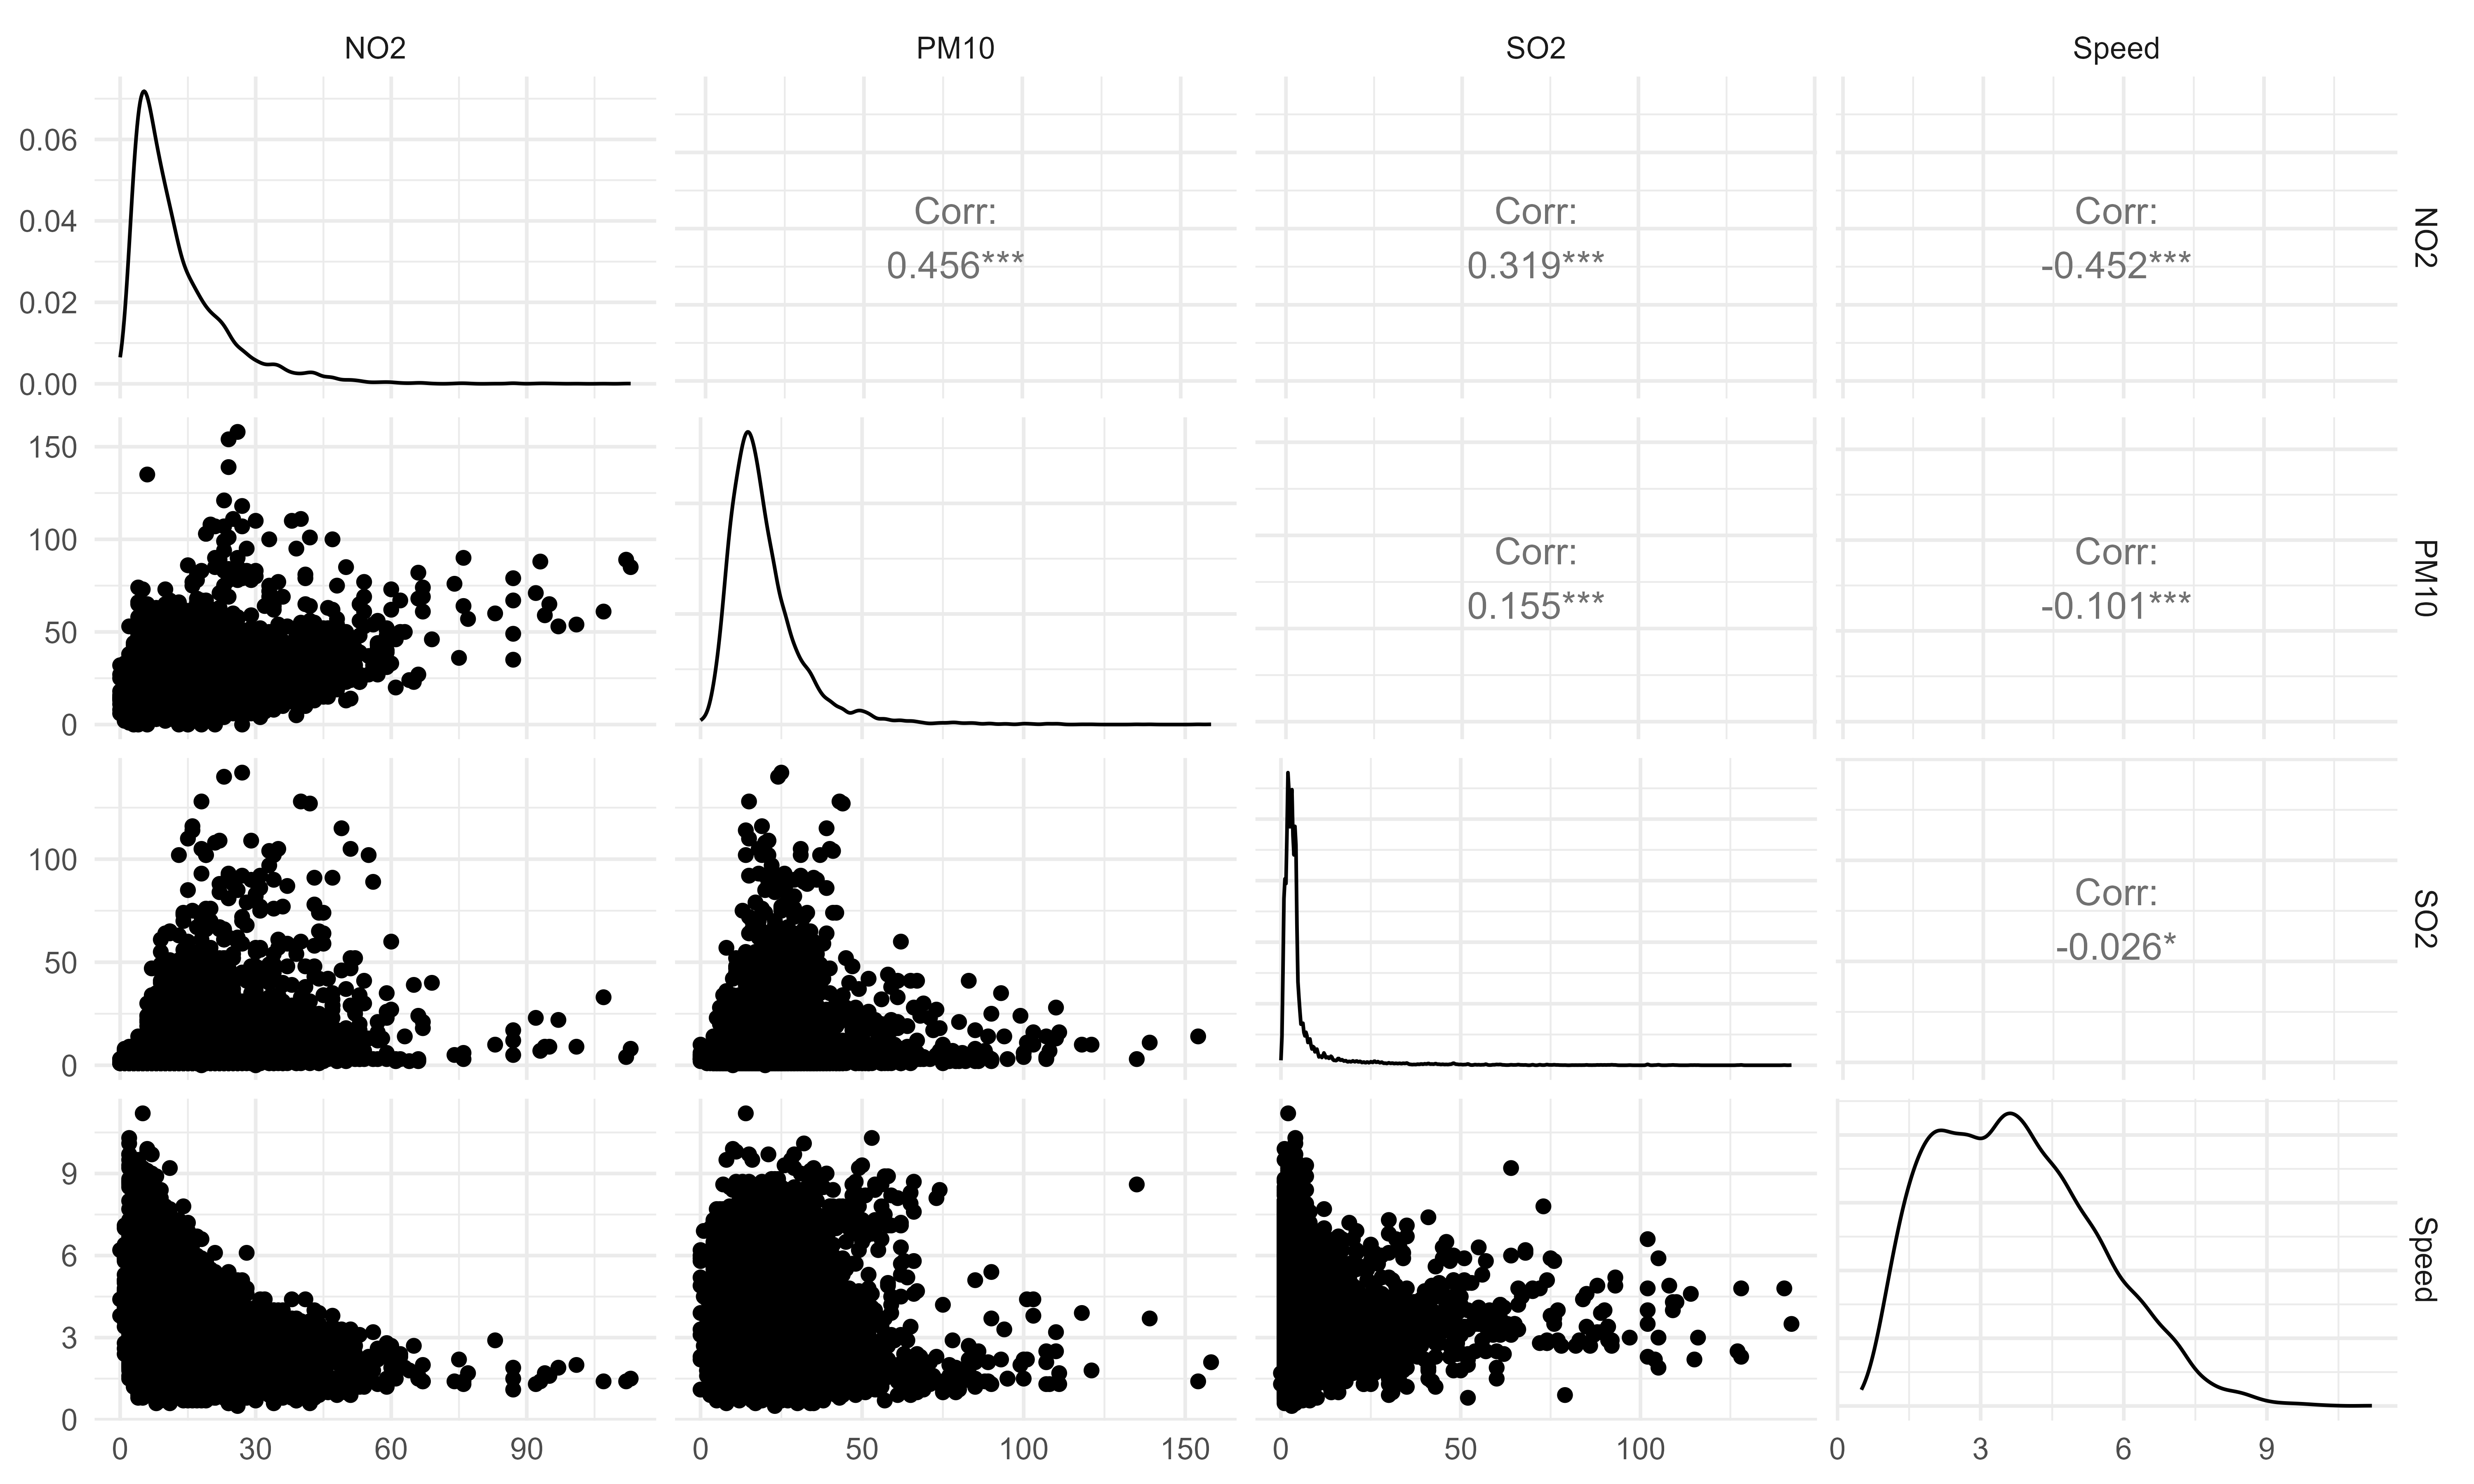
\includegraphics[width=0.48\linewidth]{../images/extracted_data_pairsplot.png}
            \caption{\textit{Pairs plot of the air quality dataset from 01/01/2019 to 31/12/2019 measured hourly.}}
         \end{figure}

         Our response variable $\text{NO}_{2}$ appears to be moderately positively correlated with $\text{PM}_{10}$ and $\text{SO}_{2}$, and moderately negatively correlated with Speed. These are not ideal explanatory variables since we typically would like them to be strongly correlated with the response variable. The explanatory variables are weakly correlated with one another, whether it be a positive or a negative correlation. This is ideal since some models do not work well with correlated explanatory variables, often leading to unstable point estimates and inflated standard errors.

         \begin{figure}[H]
            \centering
            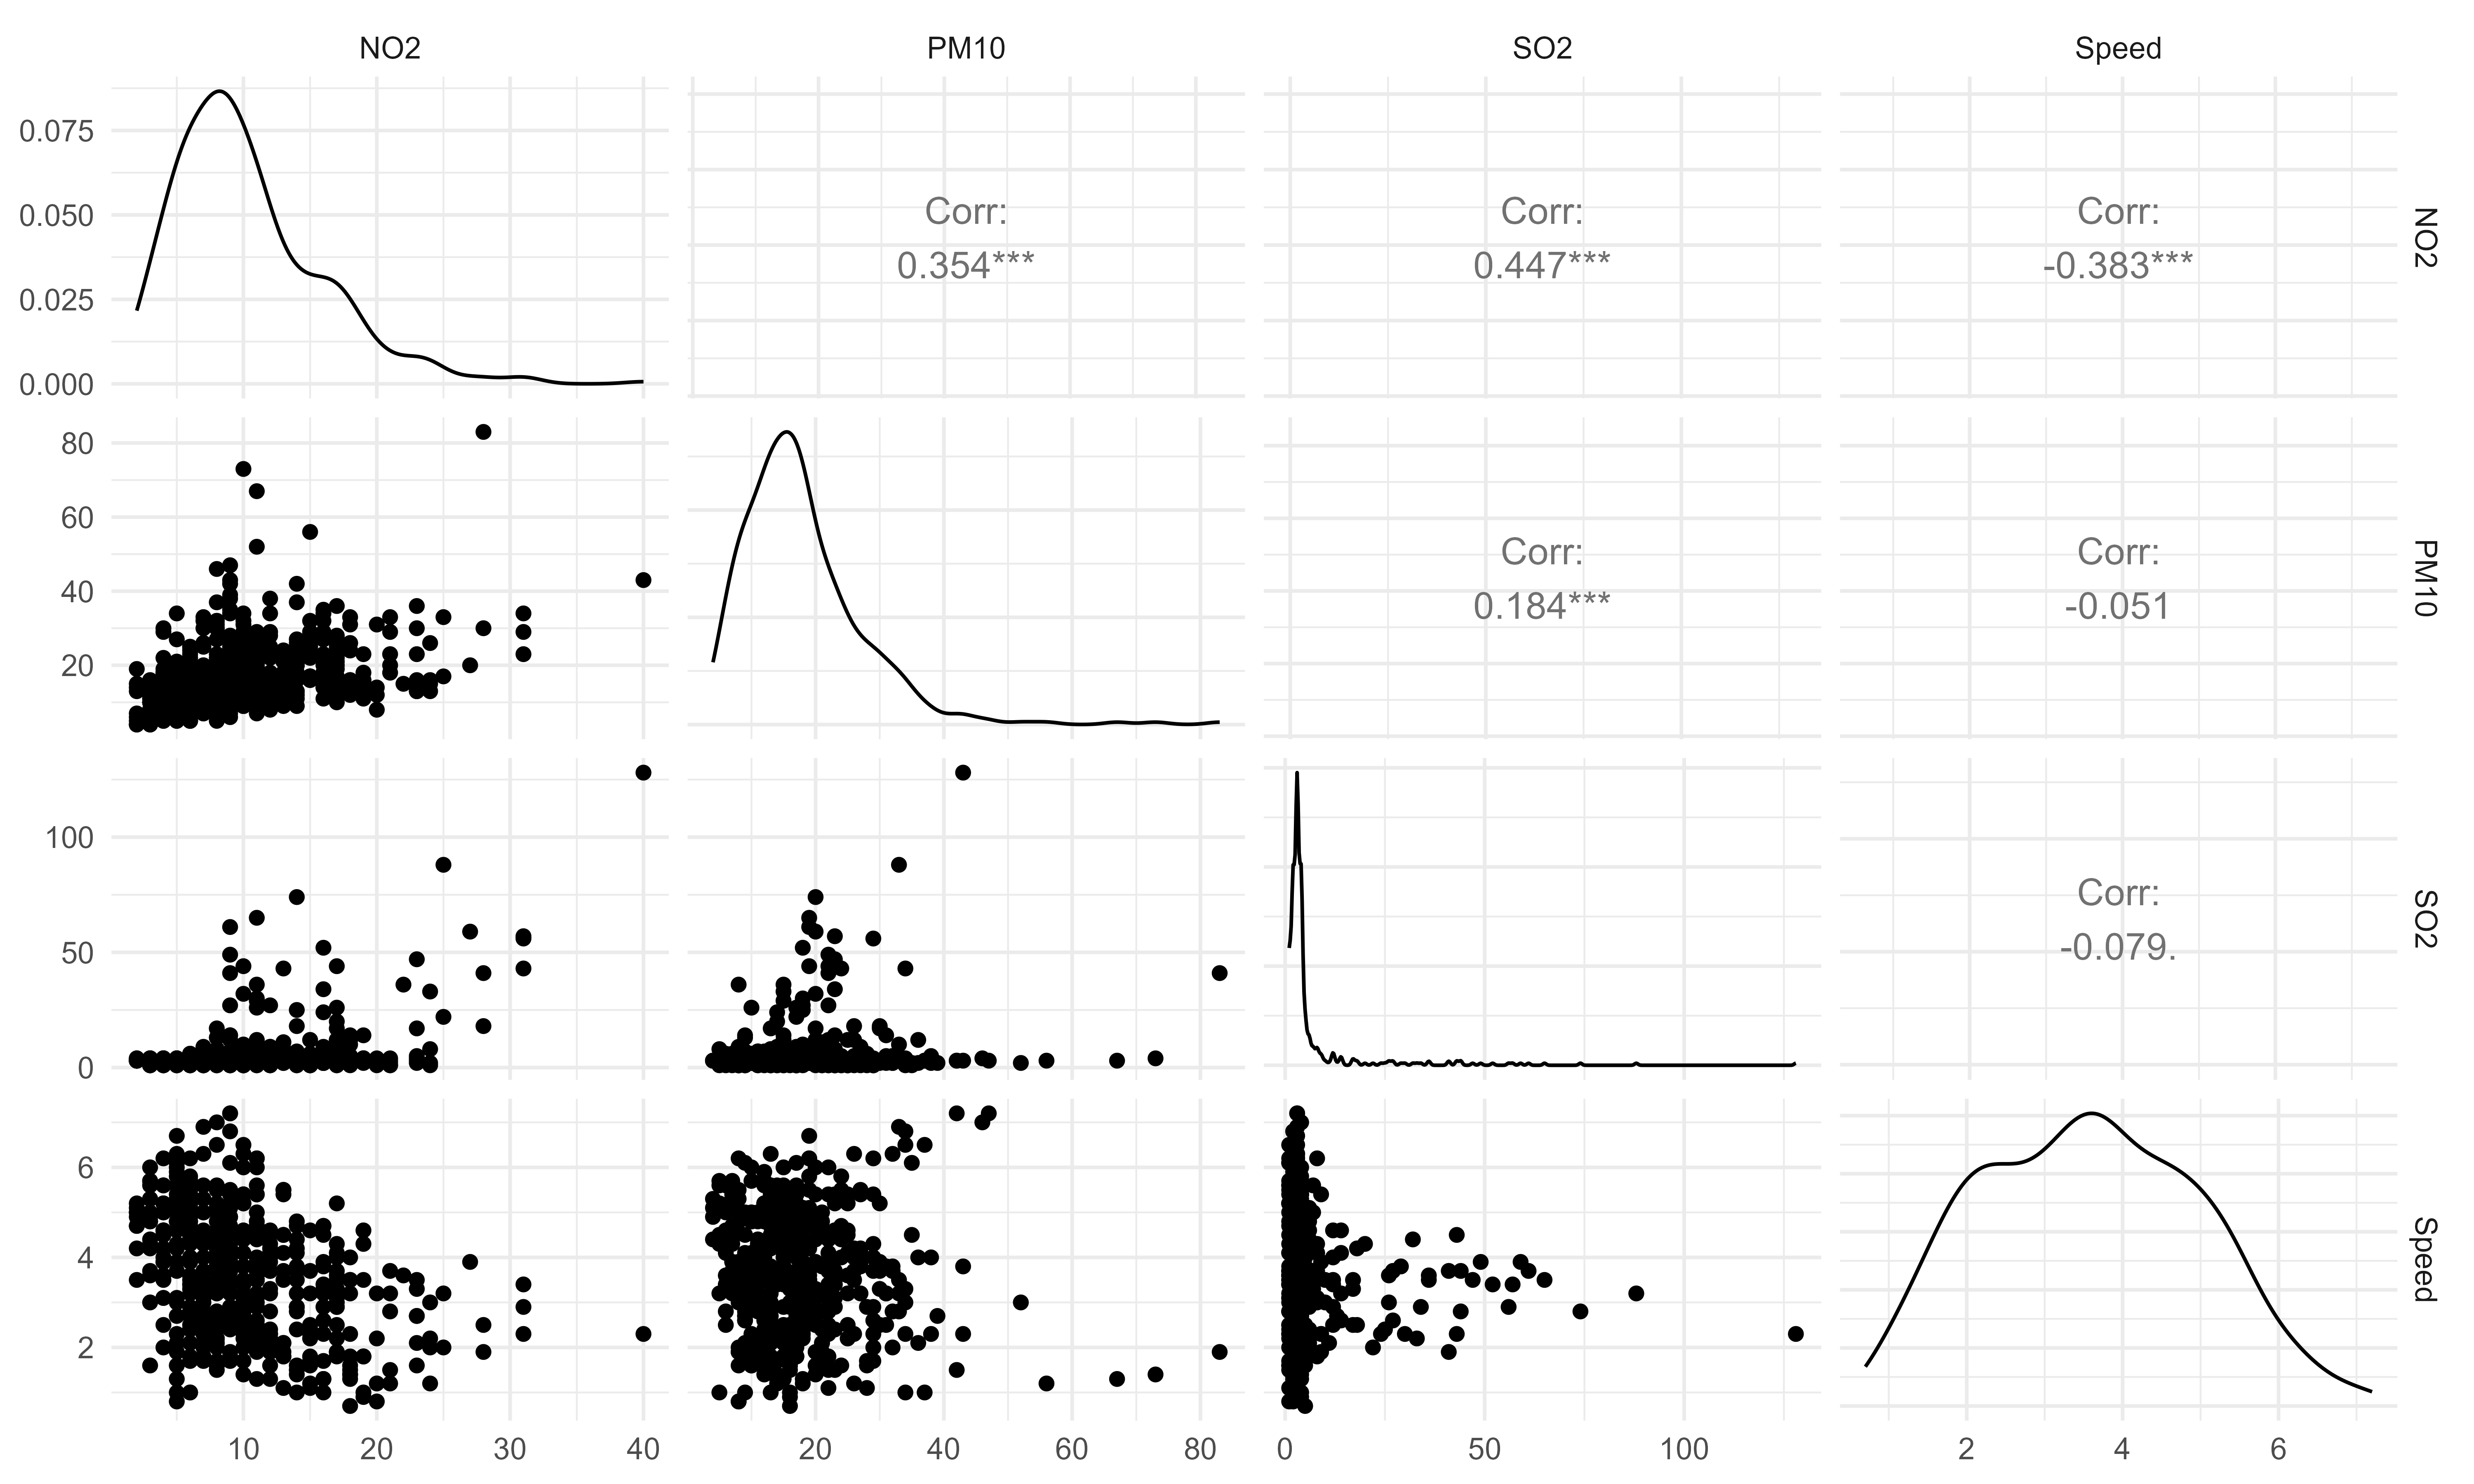
\includegraphics[width=0.48\linewidth]{../images/subset_data_pairsplot.png}
            \caption{\textit{Pairs plot of the air quality dataset from 01/01/2019 to 31/12/2019 measured hourly.}}
         \end{figure}

         \begin{figure}[H]
            \centering
            \begin{subfigure}{0.48\linewidth}
               \centering
               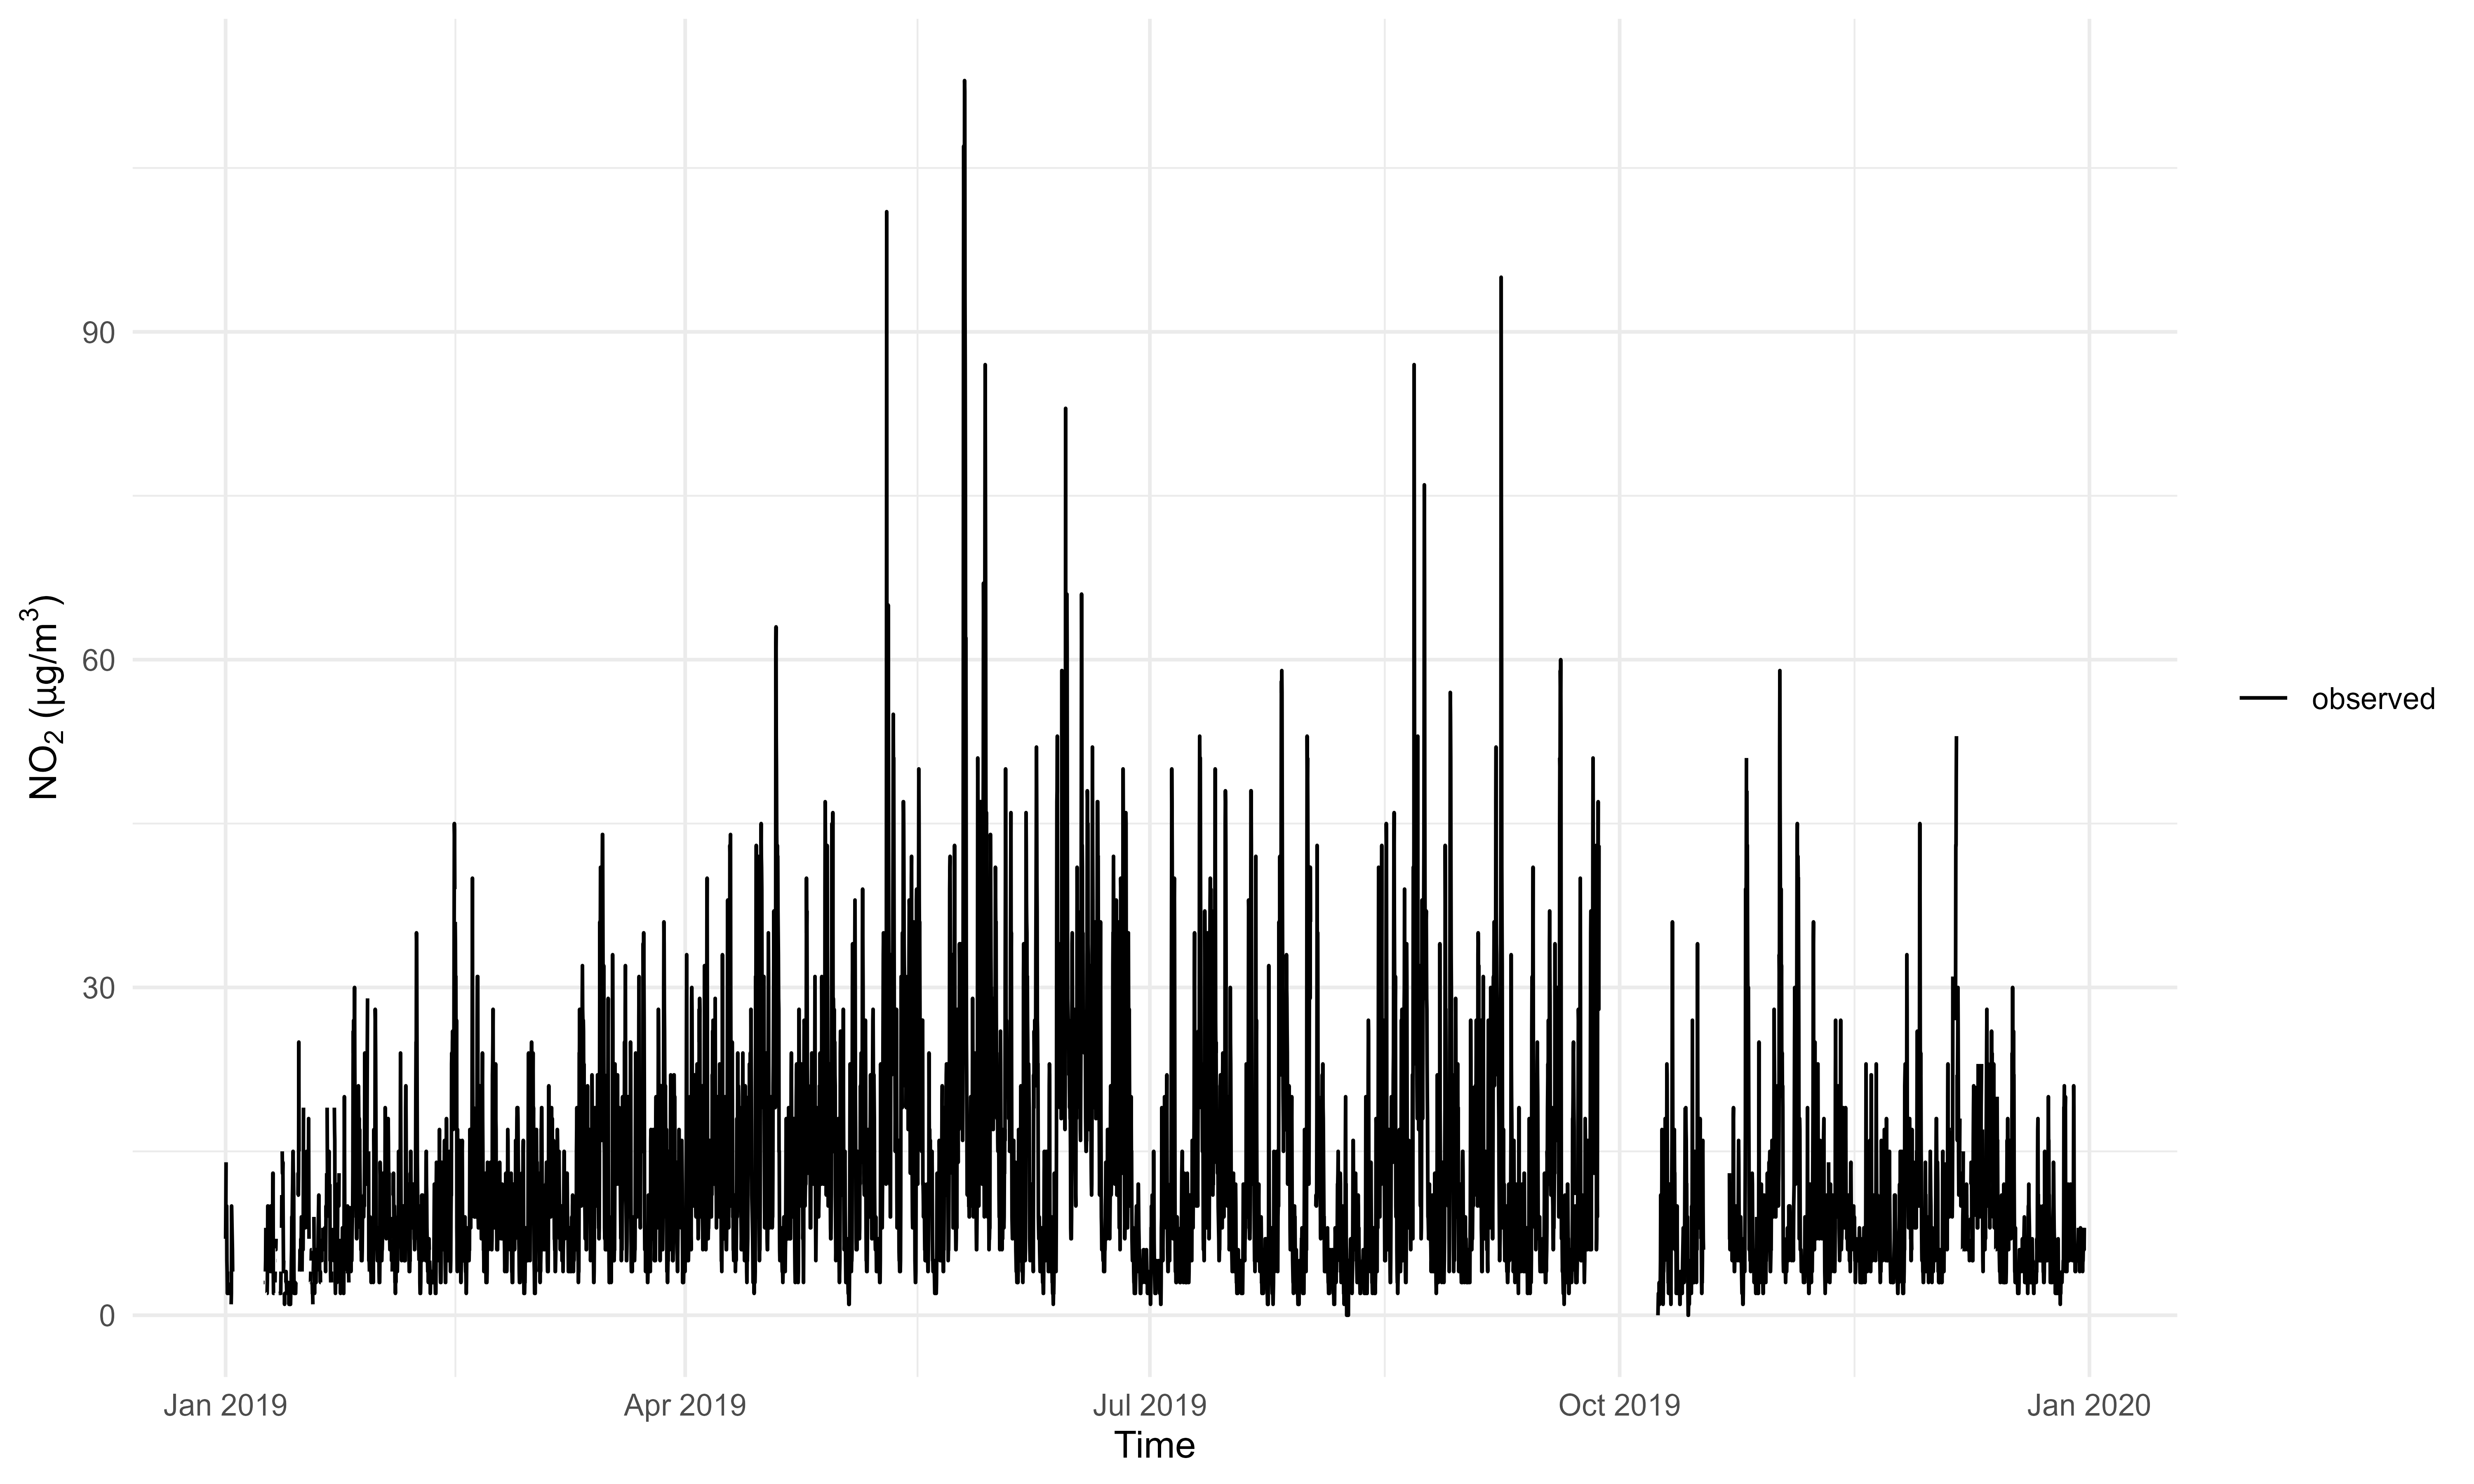
\includegraphics[width=\linewidth]{../images/extracted_data_no2.png}
            \caption{Nitrogen dioxide}
            \end{subfigure}
            \hfill
            \begin{subfigure}{0.48\linewidth}
               \centering
               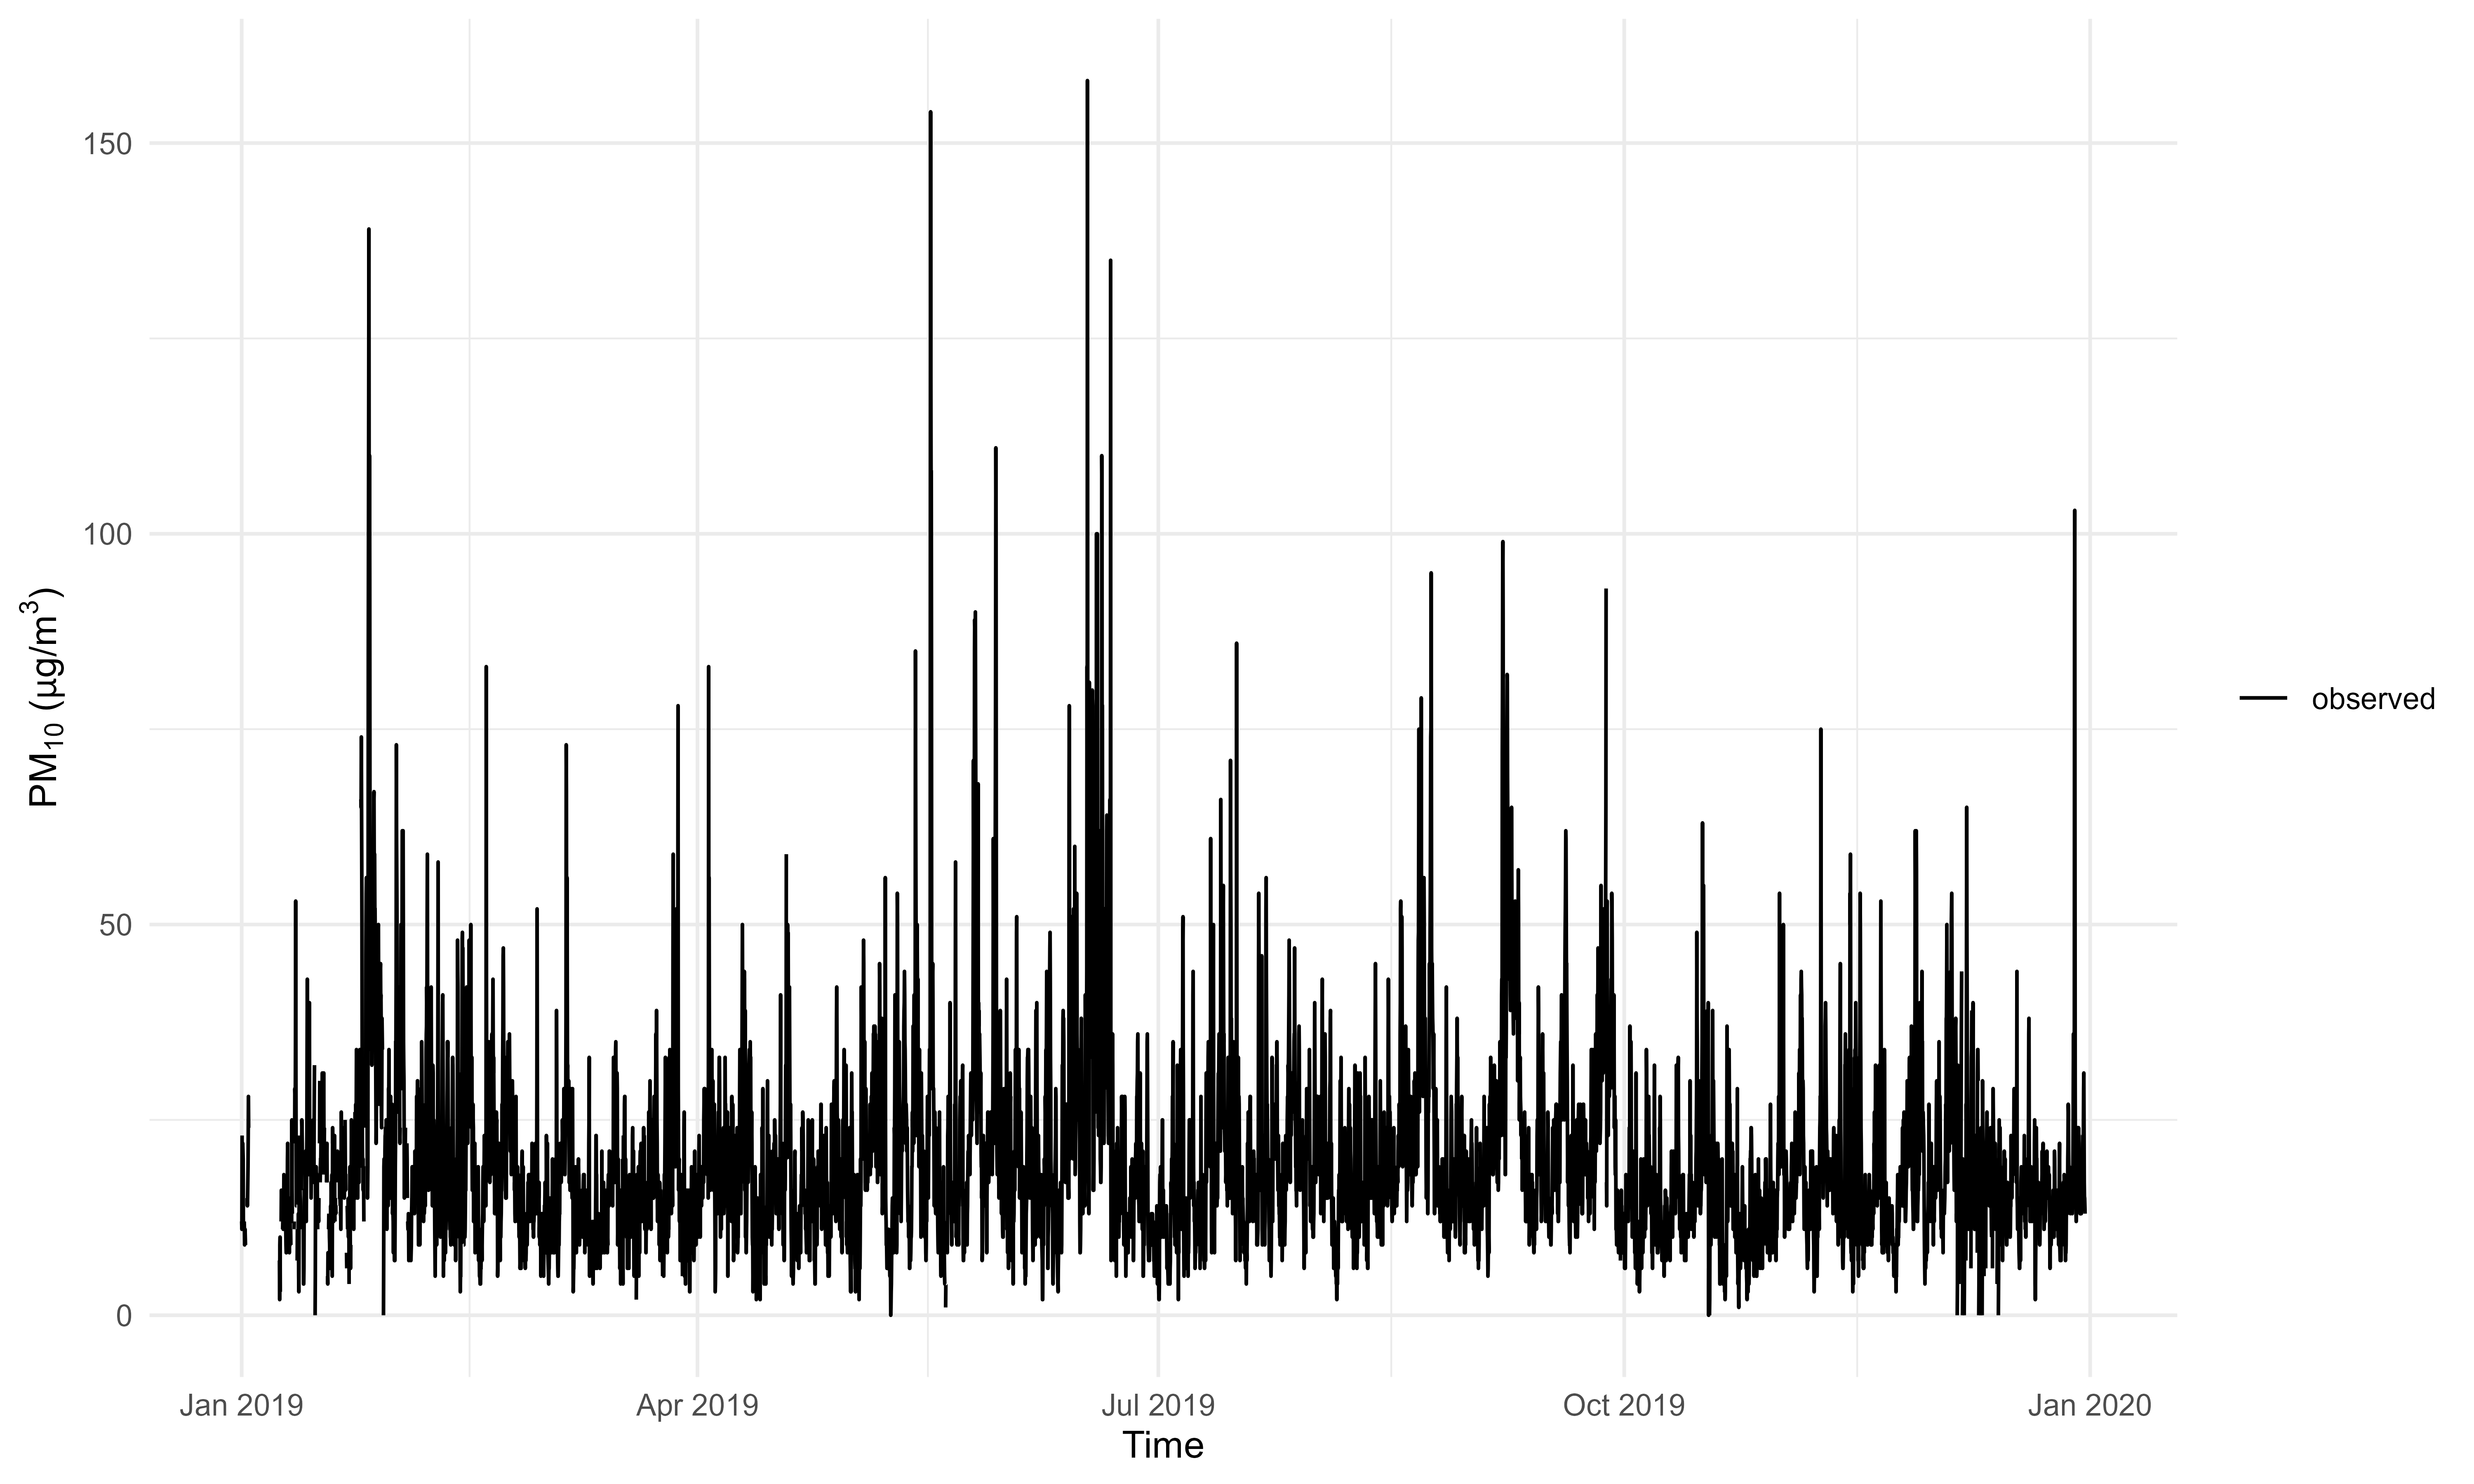
\includegraphics[width=\linewidth]{../images/extracted_data_pm10.png}
               \caption{Particulate matter 10}
            \end{subfigure}
            
            \vspace{0.5em}

            \begin{subfigure}{0.48\linewidth}
               \centering
               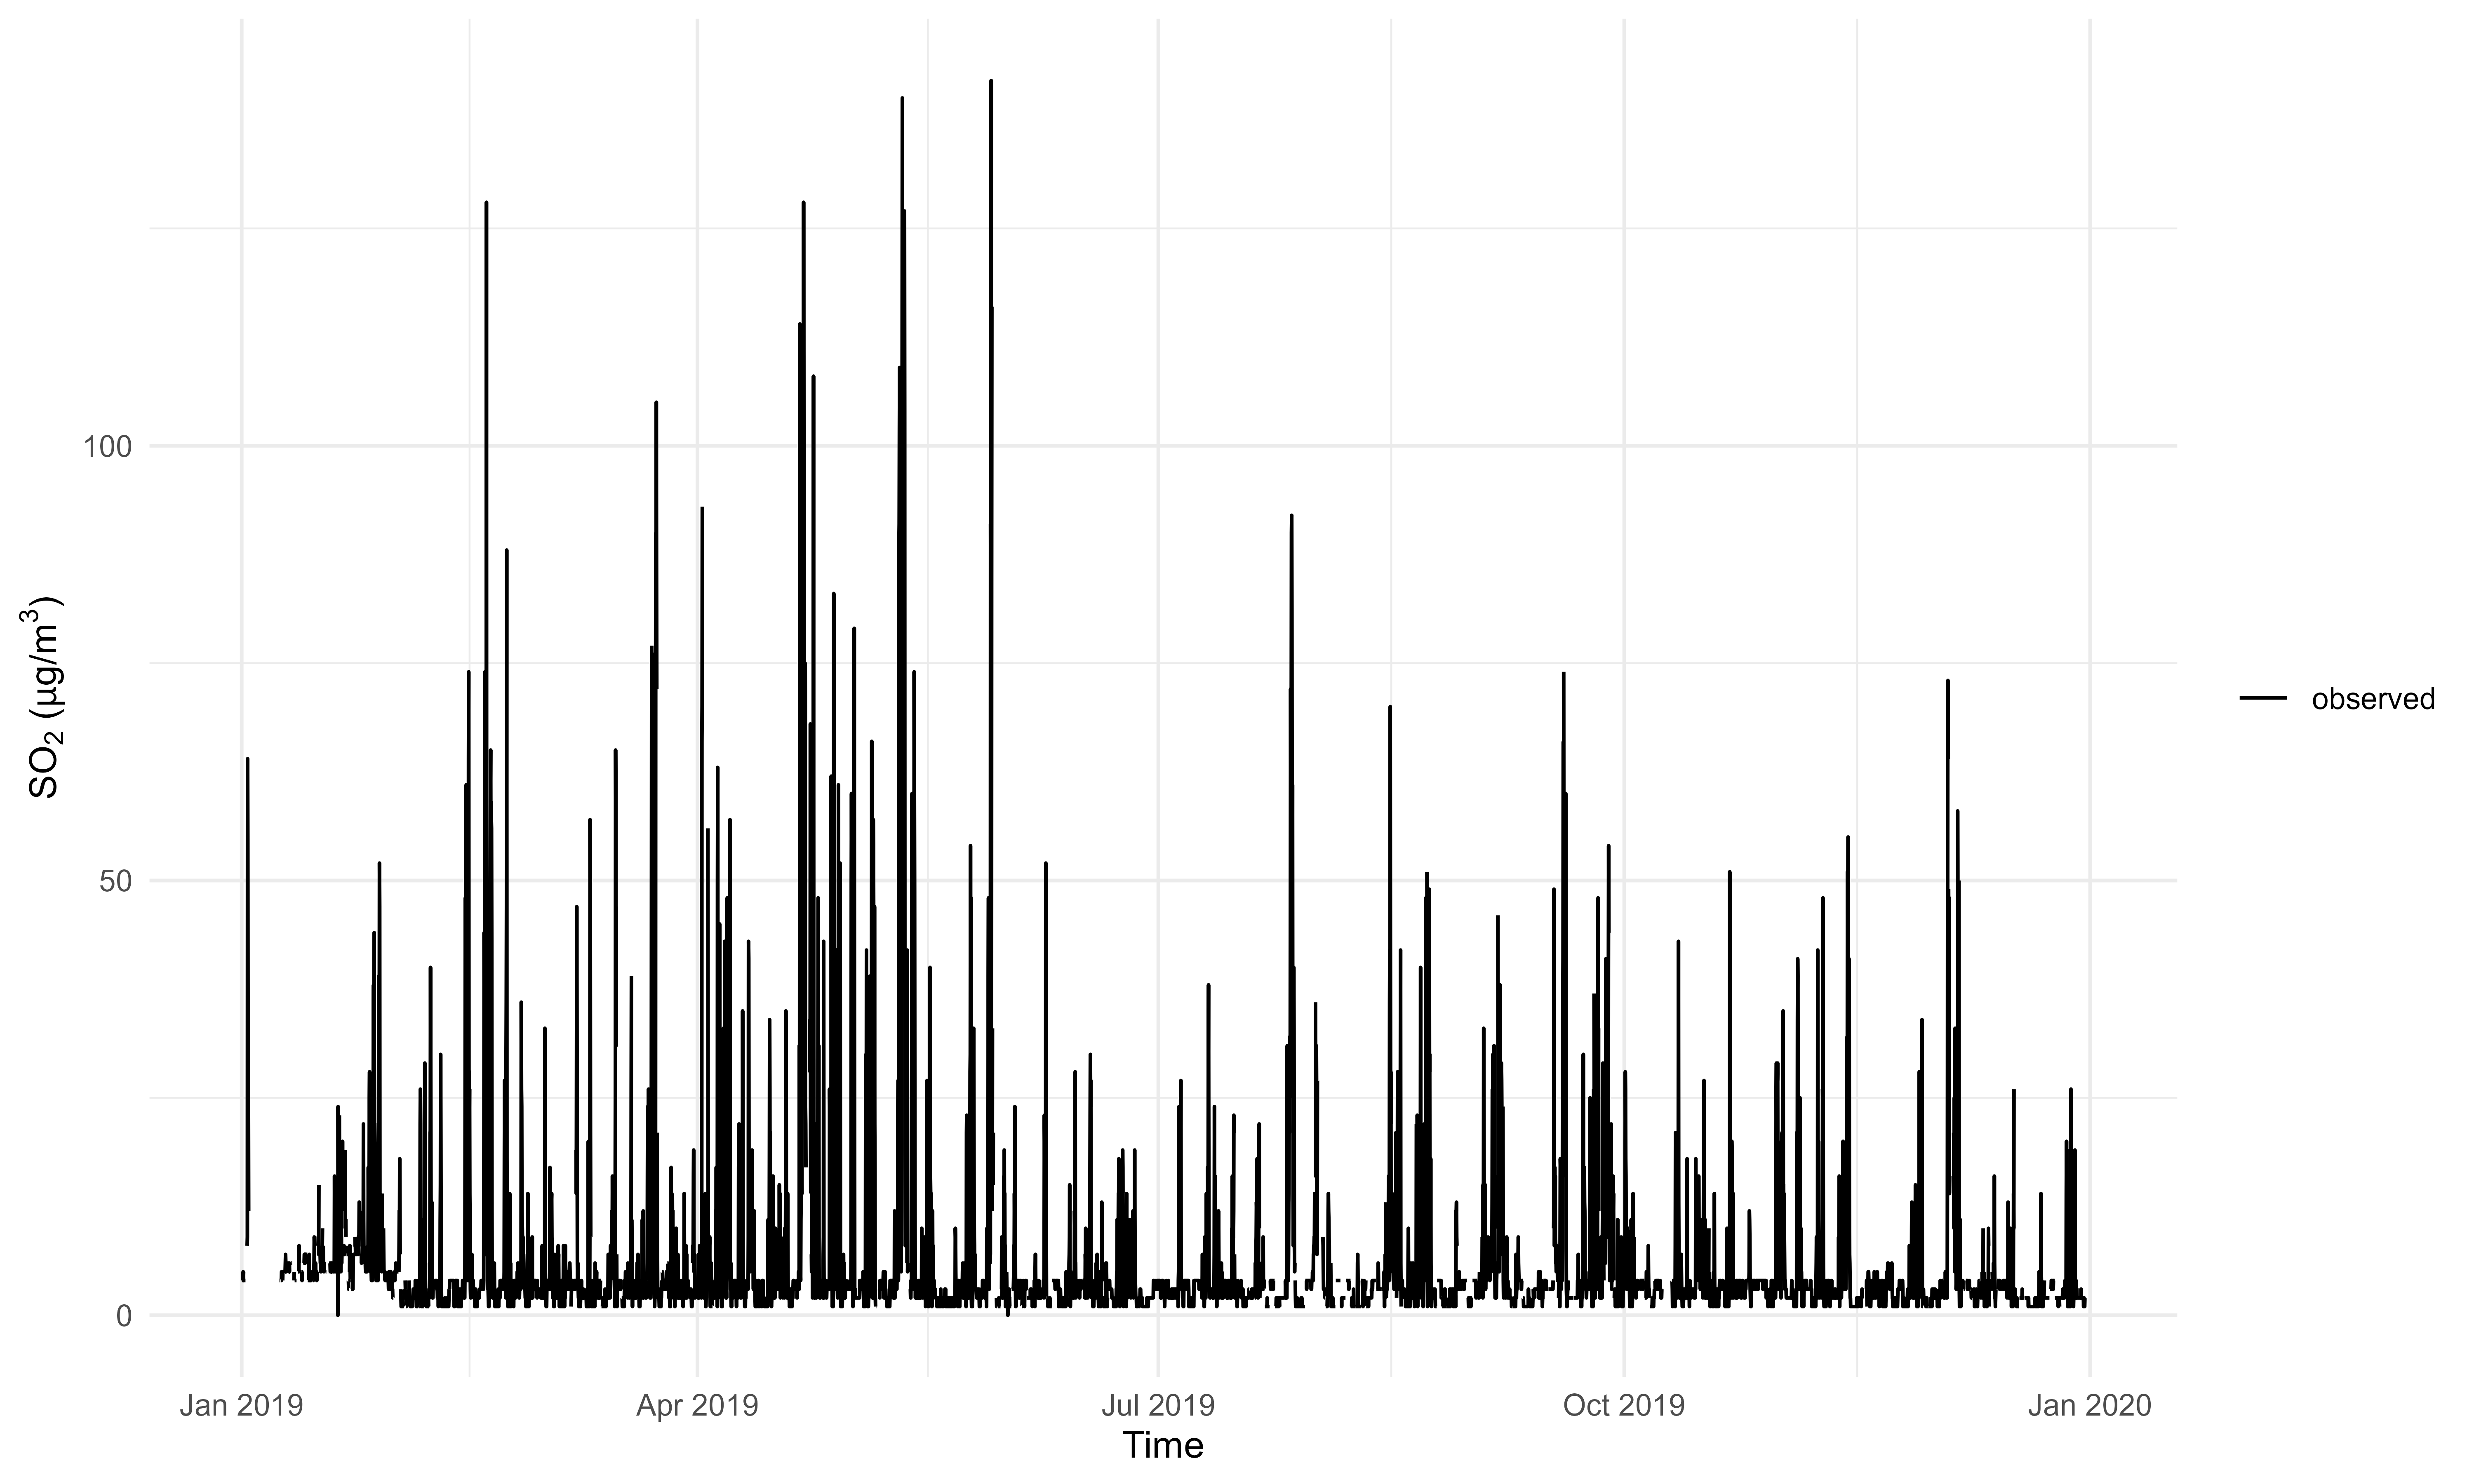
\includegraphics[width=\linewidth]{../images/extracted_data_so2.png}
            \caption{Sulphur dioxide}
            \end{subfigure}
            \hfill
            \begin{subfigure}{0.48\linewidth}
               \centering
               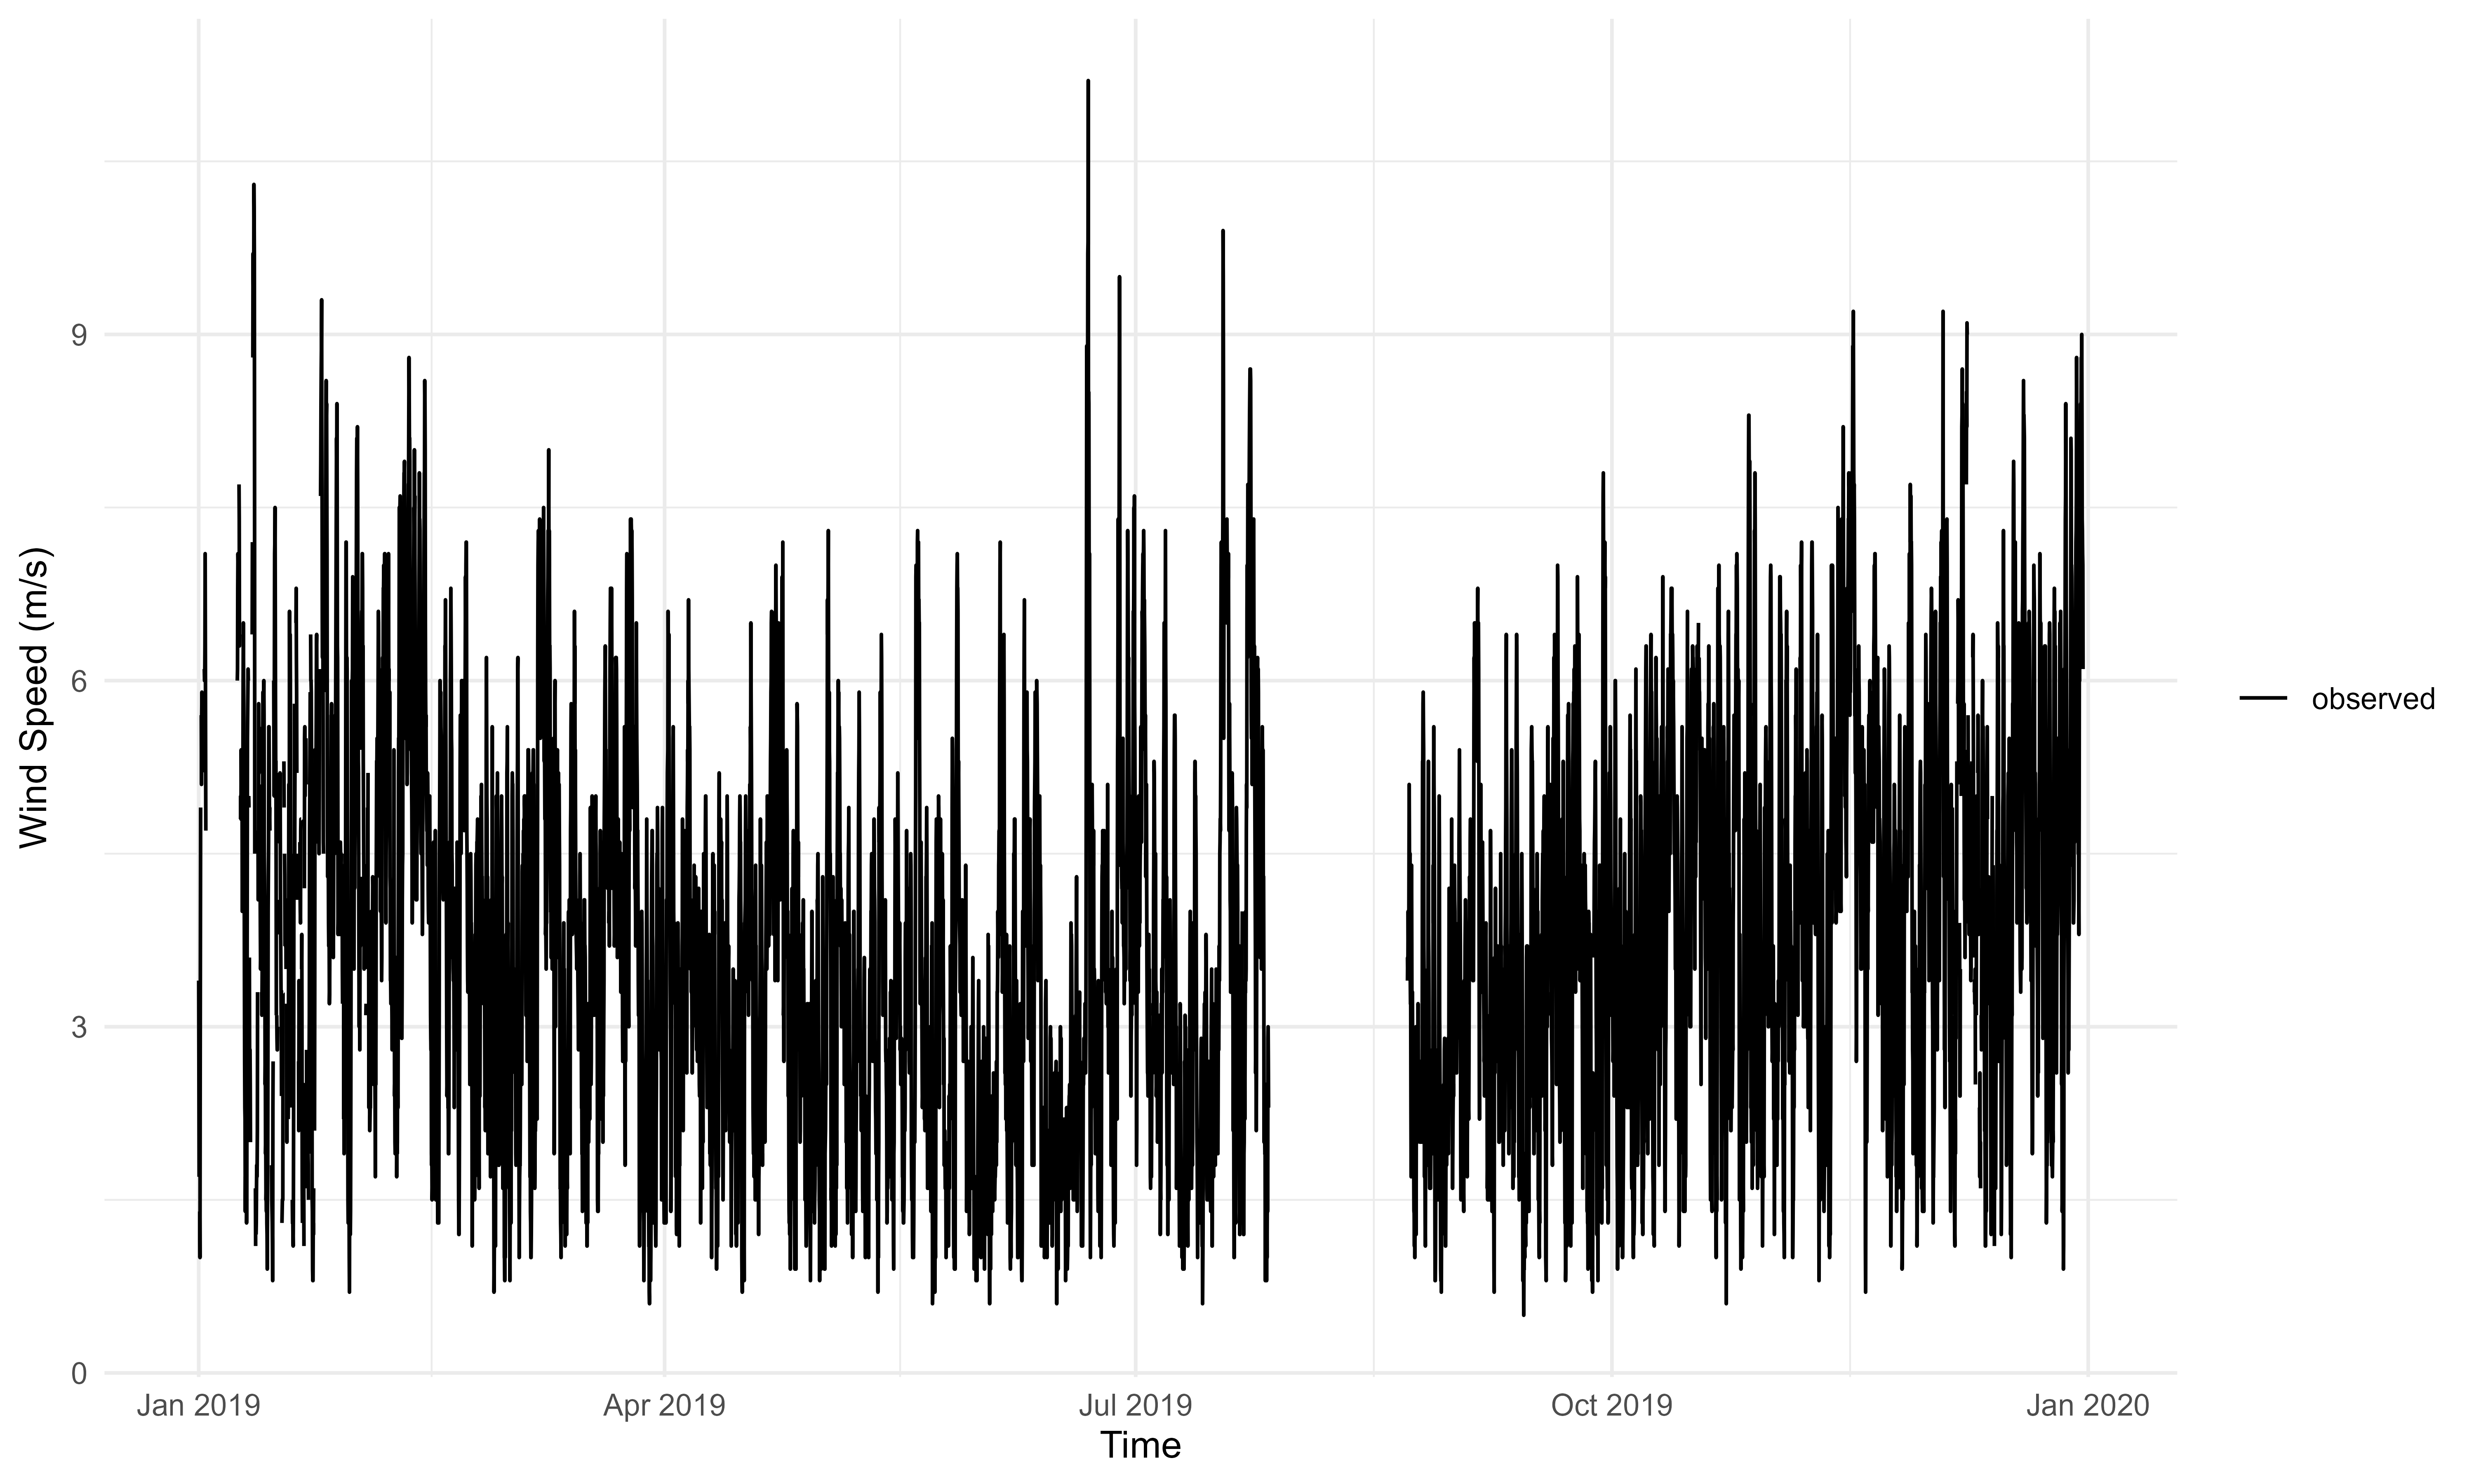
\includegraphics[width=\linewidth]{../images/extracted_data_speed.png}
               \caption{Wind speed}
            \end{subfigure}

            \caption{\textit{Time-series plots of nitrogen dioxide and meteorological processes from 01/01/2018 to 31/12/2019 measured hourly. Similar cyclic patterns can be observed in the meteorological processes, and a weaker seasonality component can be noted in the yearly nitrogen dioxide processes.}}
         \end{figure}

         There seems to be a weak seasonal and trend component based on the time series plots. There is no clear indication of a cyclical component. There is random variation as usual. It is challenging to visually identify the time series components since this is a noisy dataset.
      
         \begin{figure}[H]
            \centering
            \begin{subfigure}{0.48\linewidth}
               \centering
               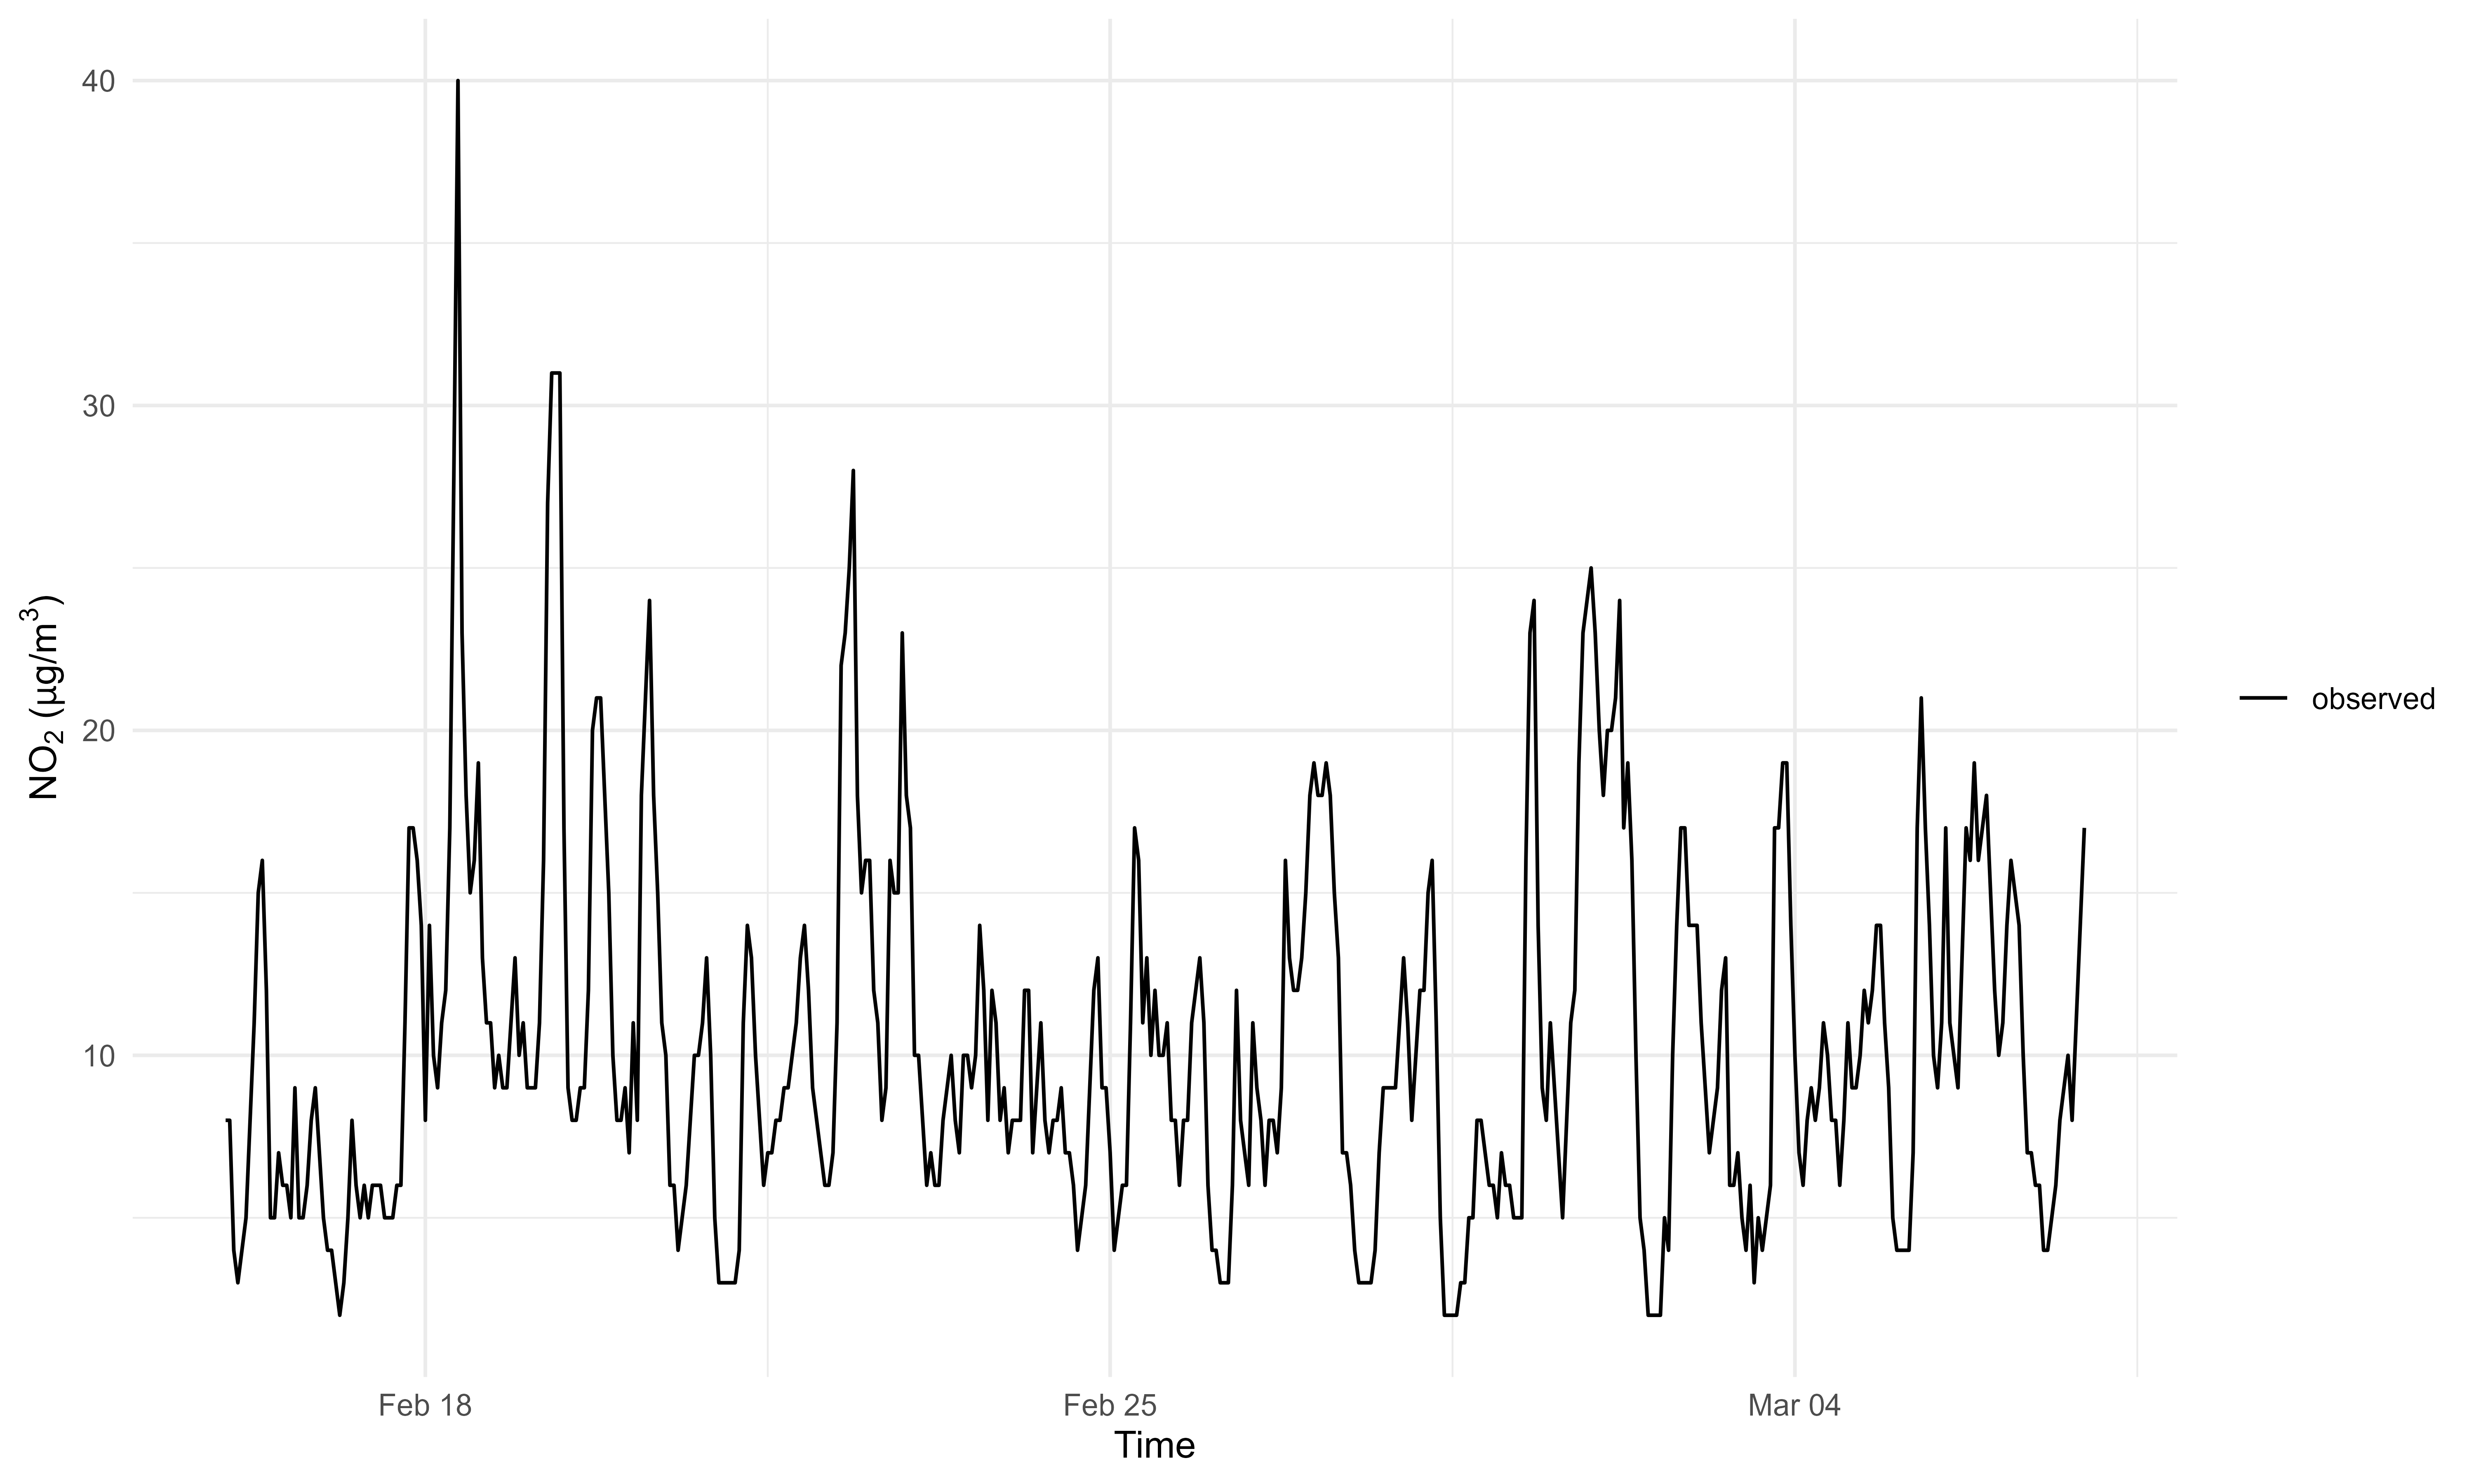
\includegraphics[width=\linewidth]{../images/subset_data_no2.png}
            \caption{Nitrogen dioxide}
            \end{subfigure}
            \hfill
            \begin{subfigure}{0.48\linewidth}
               \centering
               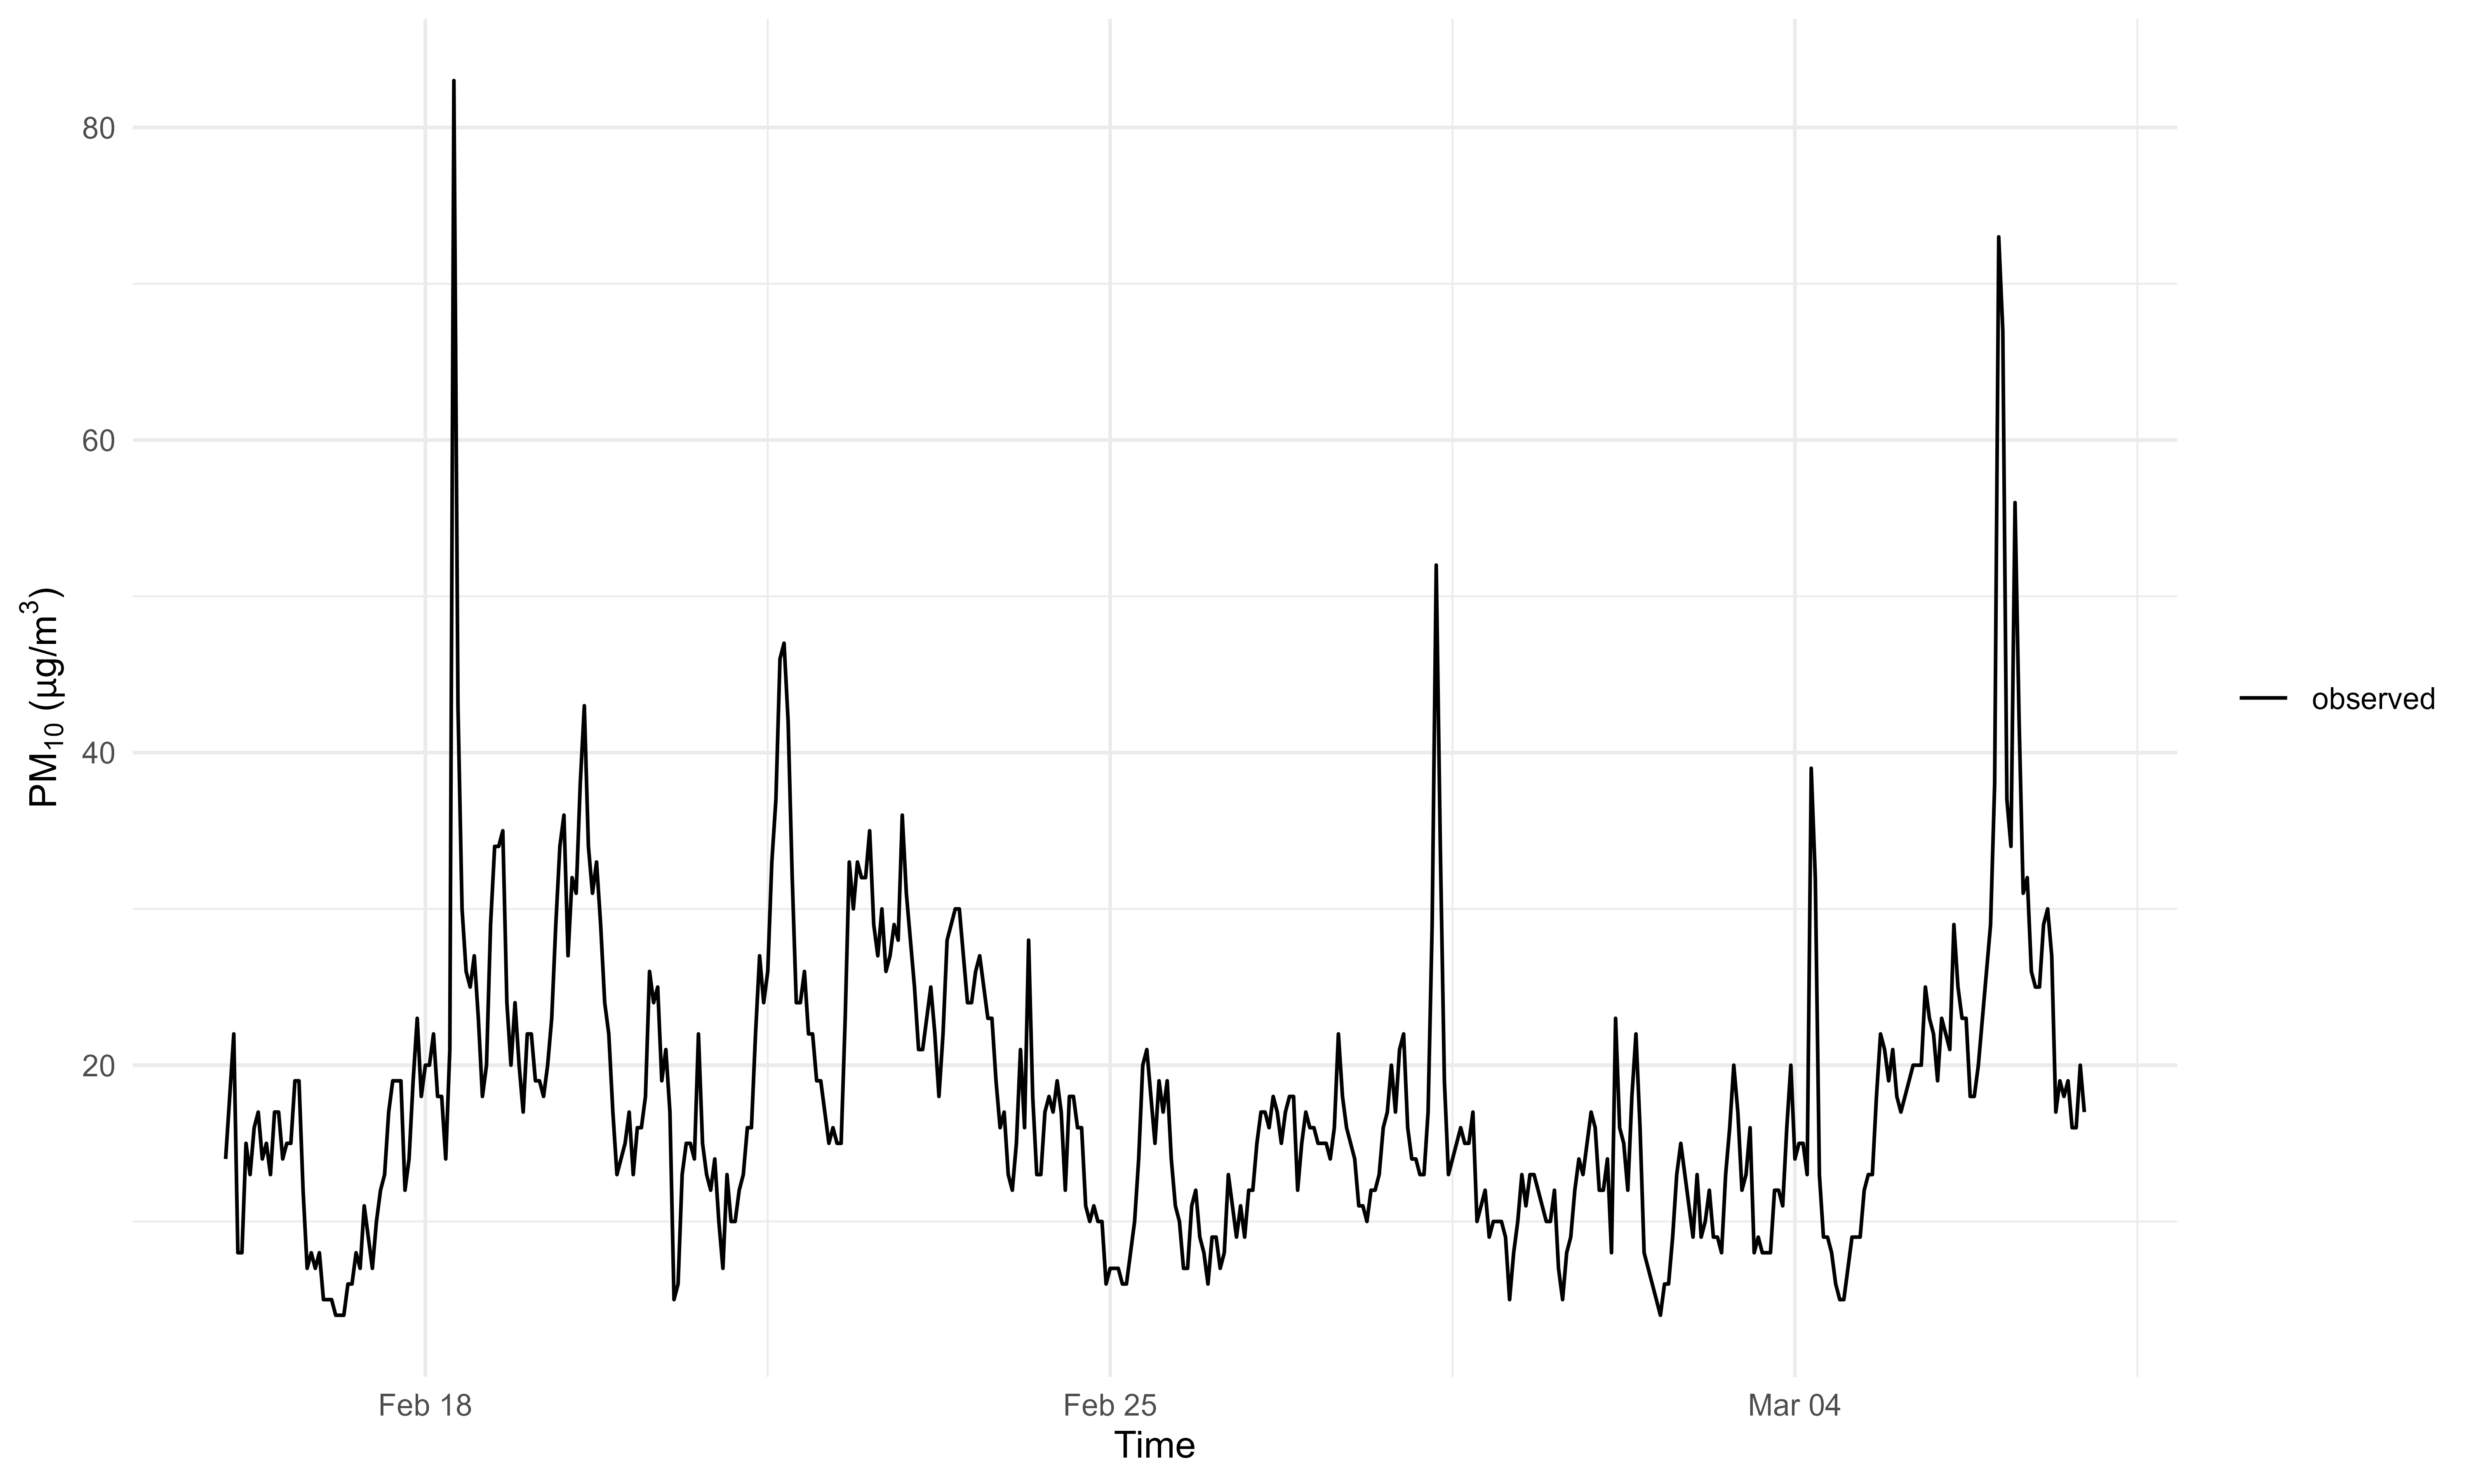
\includegraphics[width=\linewidth]{../images/subset_data_pm10.png}
               \caption{Particulate matter 10}
            \end{subfigure}
            
            \vspace{0.5em}

            \begin{subfigure}{0.48\linewidth}
               \centering
               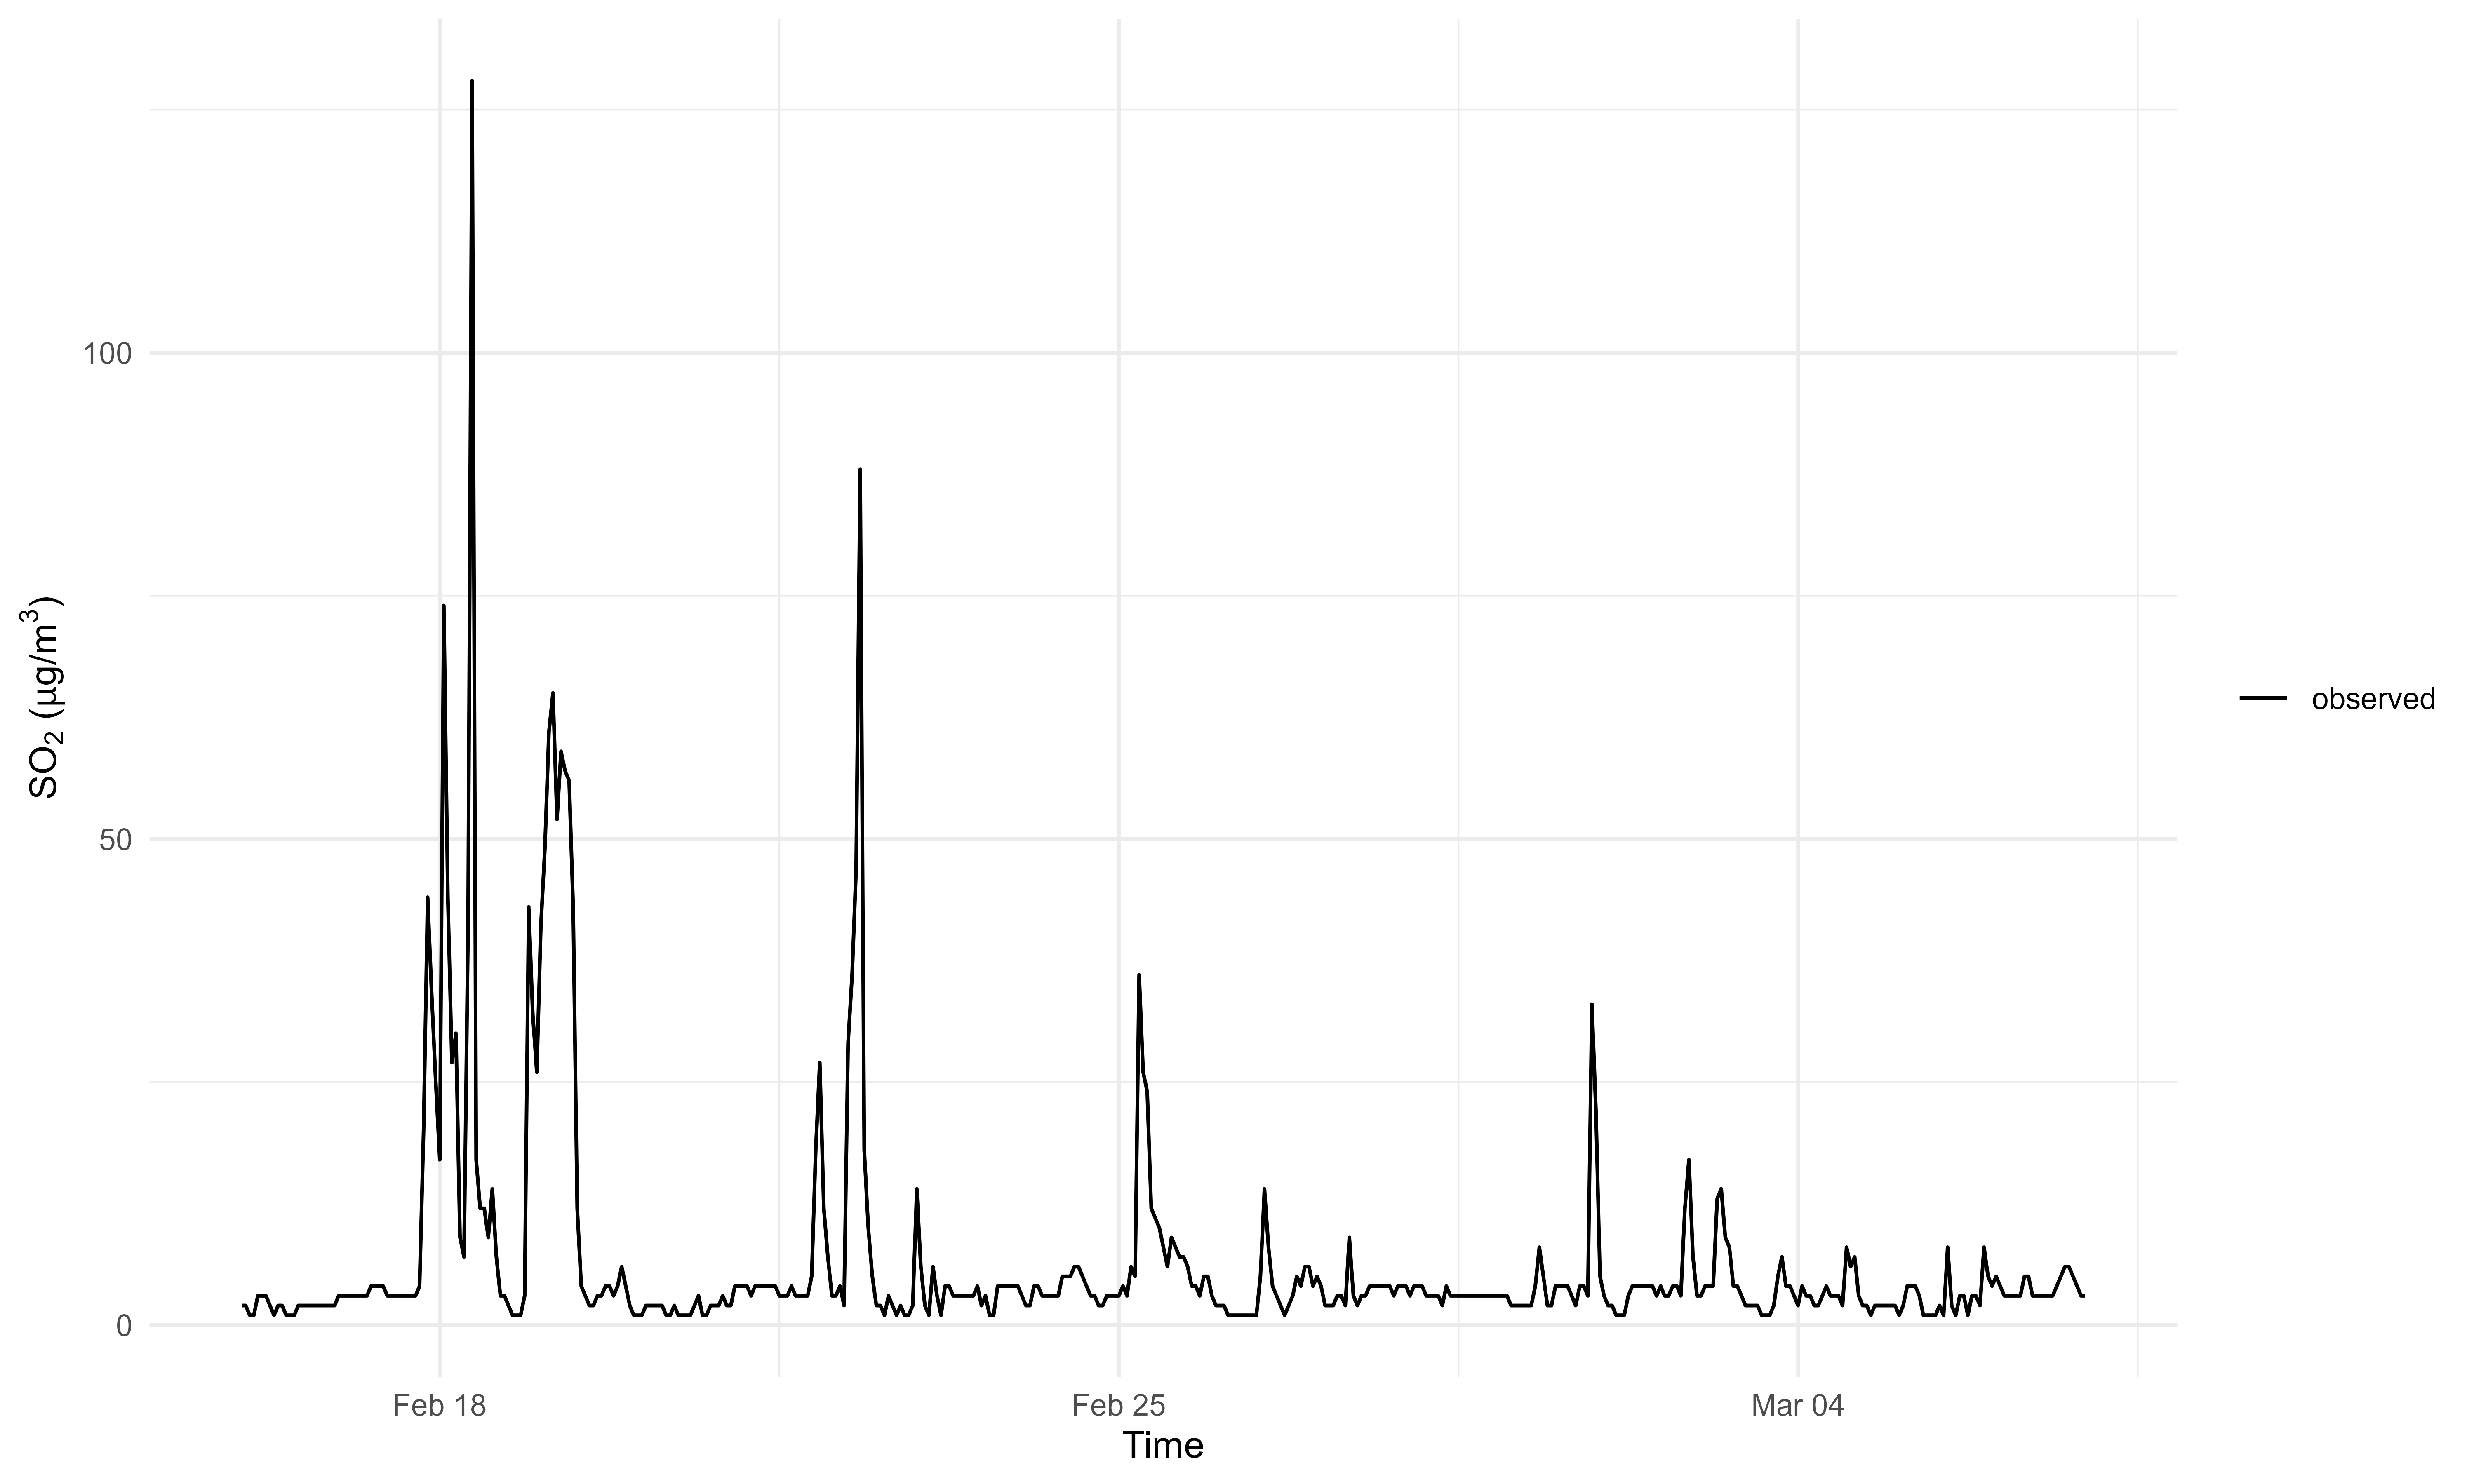
\includegraphics[width=\linewidth]{../images/subset_data_so2.png}
            \caption{Sulphur dioxide}
            \end{subfigure}
            \hfill
            \begin{subfigure}{0.48\linewidth}
               \centering
               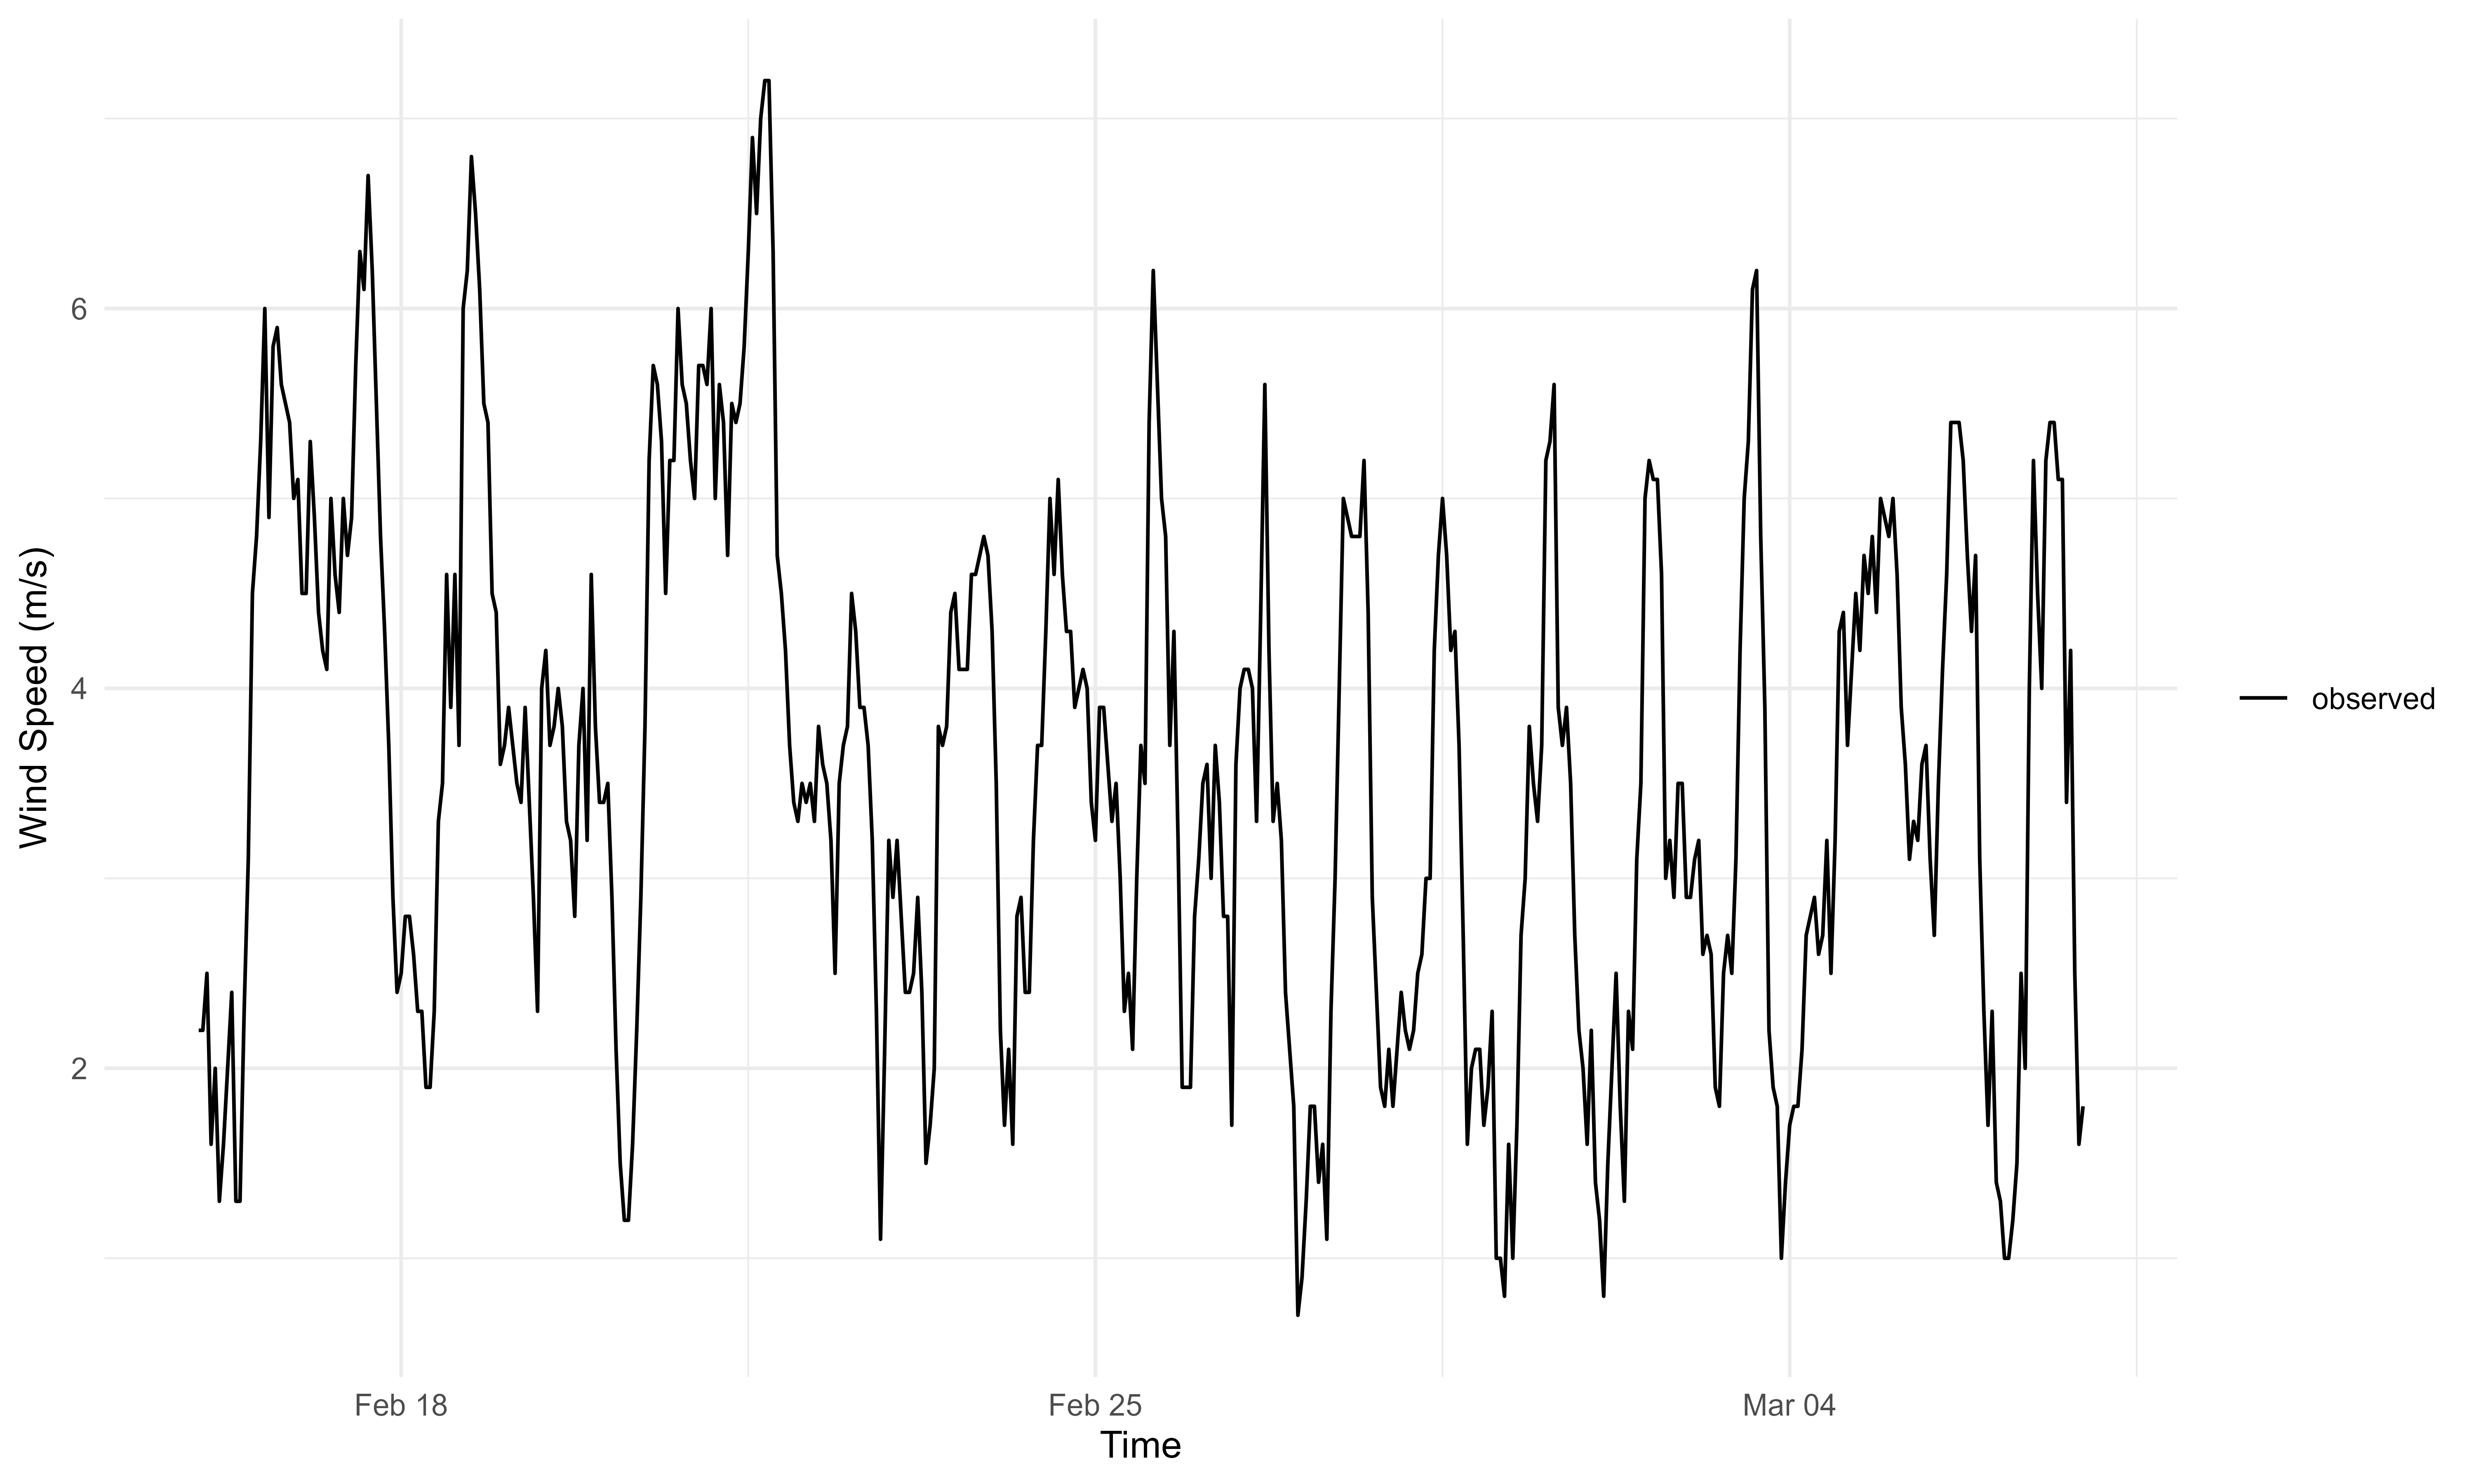
\includegraphics[width=\linewidth]{../images/subset_data_speed.png}
               \caption{Wind speed}
            \end{subfigure}

            \caption{\textit{Time-series plots of nitrogen dioxide and meteorological processes from 15/02/2019 at 23:00:00 to 06/03/2019 at 23:00:00 measured hourly. Similar cyclic patterns can be observed in the meteorological processes, and a weaker seasonality component can be noted in the yearly nitrogen dioxide processes.}}
         \end{figure}

   \subsection{Methodology}
   
      $$y \sim \text{GP}(m(\cdot),\, k(\cdot,\, \cdot))$$

      Linear mean function:

      $$m(x_{i}) = \sum_{j=1}^{p} x_{ij}\beta_{j}, \quad \text{where} \quad i \in \{1,\, \ldots,\, \text{n}\}.$$

      The resulting mean vectors of the training set and test set respectively are as follows.

      $$\mathbf{m}_{1} = \mathbf{X}_{1}\boldsymbol{\beta}$$
      $$\mathbf{m}_{2} = \mathbf{X}_{2}\boldsymbol{\beta}$$
      Squared-exponential kernel:
      $$k(x_{i},\, x_{j}) = \alpha^2 \text{exp} \bigg(-\frac{(x_{i} - x_{j})^2}{2\rho^2} \bigg) + \delta\text{I}_{i=j}, \, \text{where} \, \alpha,\, \rho \text{ are hyperparameters and } \delta = 1\text{e}-9.$$
      The resulting covariance matrices are as follows
      $$\mathbf{K}_{11} = k(\mathbf{X}_{1},\, \mathbf{X}_{1}) + \delta\mathbf{I}_{n_{1}}$$
      $$\mathbf{K}_{12} = k(\mathbf{X}_{1},\, \mathbf{X}_{2})$$
      $$\mathbf{K}_{22} = k(\mathbf{X}_{2},\, \mathbf{X}_{2}) + \delta\mathbf{I}_{n_{2}}$$
      The likelihood is the following.
      $$\mathbf{y}_{1}|\, \boldsymbol{\beta}, \alpha, \rho \sim \mathcal{N}(\mathbf{m}_{1},\, \mathbf{K}_{11})$$

      Choosing the following priors.
      $$\boldsymbol{\beta} \sim \mathcal{N}(0,\, \mathbf{I}_{p})$$
      $$\alpha \sim \text{half-normal}(0, 1)$$
      $$\rho \sim \text{half-normal}(24,\, 12)$$
      The joint distribution of $[\mathbf{y}_{1},\, \mathbf{y}_{2}]$ given fixed parameters $(\boldsymbol{\beta},\, \alpha,\, \rho)$, the joint distribution of the training and set outputs is a multivariate normal:
      $$\begin{bmatrix} \mathbf{y}_{1} \\ \mathbf{y}_{2} \end{bmatrix} \sim \mathcal{N} \Bigg(\begin{bmatrix} \mathbf{m}_{1} \\ \mathbf{m}_{2} \end{bmatrix},\, \begin{bmatrix} \mathbf{K}_{11} & \mathbf{K}_{12} \\ \mathbf{K}_{21} & \mathbf{K}_{22} \end{bmatrix} \Bigg).$$
      The conditional distribution of $\mathbf{y}_{2}|\, \mathbf{y}_{1},\, \boldsymbol{\beta},\, \alpha,\, \rho$. This is just a conditional distribution of a multivariate normal distribution which is a well known result.
      $$\mathbf{y}_{2}|\, \mathbf{y}_{1},\, \boldsymbol{\beta},\, \alpha,\, \rho \sim \mathcal{N}(\mathbf{m}_{2} + \mathbf{K}_{12}^{\text{T}}\mathbf{K}_{11}^{-1}(\mathbf{y}_{1} - \mathbf{m}_{1}),\, \mathbf{K}_{22} - \mathbf{K}_{12}^{\text{T}} \mathbf{K}_{11}^{-1} \mathbf{K}_{12})$$
      $$\pi(\mathbf{y}_{2}|\, \mathbf{y}_{1}) = \int \pi(\mathbf{y}_{2}|\, \mathbf{y}_{1},\, \boldsymbol{\beta},\, \alpha,\, \rho) \, \pi(\boldsymbol{\beta}) \, \pi(\alpha) \, \pi(\rho) \,  d\boldsymbol{\beta}\, d\alpha\, d\rho.$$
      This does not have a closed form solution. We approximated the posterior samples of this distribution using `Stan`. `Stan` avoids computing explicit inverses. These quantities are calculated in `Stan` as follows.

      Cholesky decomposition of $\mathbf{K}_{11}$. 
      $$\mathbf{K}_{11} = \mathbf{L} \mathbf{L}^{\text{T}}.$$

      Compute $\mathbf{w} = \mathbf{K}_{11}^{-1}(\mathbf{y}_{1} - \mathbf{m}_{1})$ via triangular solves:
      $$\mathbf{v} = \mathbf{L}^{-1}(\mathbf{y}_{1} - \mathbf{m}_{1}).$$
      Then $$\mathbf{w} = (\mathbf{L}^{\text{T}})^{-1} \mathbf{v}.$$
      Thus $$\mathbf{w} = \mathbf{K}_{11}^{-1}(\mathbf{y}_{1} - \mathbf{m}_{1}).$$

      The predictive mean is calculated as follows. 

      $$\mathbf{m}_{2} + \mathbf{K}_{12}^{\text{T}}\mathbf{w} = \mathbf{m}_{2} + \mathbf{K}_{12}^{\text{T}}\mathbf{K}_{11}^{-1}(\mathbf{y}_{1} - \mathbf{m}_{1}).$$
      And the predictive covariance is calculated as follows.

      $$\mathbf{A} = \mathbf{L}^{-1} \mathbf{K}_{12}.$$
      Then $$\mathbf{A}^{\text{T}} \mathbf{A} = \mathbf{K}_{12}^{\text{T}} \mathbf{L}^{-\text{T}} \mathbf{L}^{-1} \mathbf{K}_{12}.$$
      Thus $$\mathbf{A}^{\text{T}} \mathbf{A} = \mathbf{K}_{12}^{\text{T}} \mathbf{K}_{11}^{-1} \mathbf{K}_{12}.$$

      Then draw samples from $\mathbf{y}_{2}|\, \mathbf{y}_{1}$ via Hamiltonian Monte Carlo (HMC) in `Stan`. The algorithm proceeds as follows.

      1. `Stan` samples the parameters $(\boldsymbol{\beta},\, \alpha,\, \rho)$ from the posterior distribution $\pi(\boldsymbol{\beta},\, \alpha,\, \rho|\, \mathbf{y}_{1})$ using HMC.

      2. For each parameter draw `Stan` then executes the `generated quantities` block which:
      - Computes the predictive mean and predictive covariance,
      - draws $$\mathbf{y}_{2}^{(s)} \sim \mathcal{N}(\text{pred mean},\, \text{pred covariance})$$ using `multi_normal_rng`. 
         The RNG draw is not part of the HMC dynamics - it happens after the sampler proposes/accepts a parameter sample.

      3. Collecting the $\mathbf{y}_{2}^{(s)}$ across all saved iterations gives a Monte Carlo approximation to the marginal posterior predictive $$\pi(\mathbf{y}_{2}|\, y_{1}) \approx \frac{1}{S} \sum_{s=1}^{S} \mathcal{N}(\mathbf{y}_{2}|\, \mu^{(s)},\, \Sigma^{(s)}),$$ where $\mu^{(s)},\, \Sigma^{(s)}$ are conditional mean/covariance computed at the $s$-th parameter draw.
   
   \subsection{Cross-validation}

      Cross-validation was conducted as follows: a period of 7 days from 08/02/2019 at 00:00 to 15/02/2019 at 23:00 was used for the training set, and 1 day from 16/02/2019 at 00:00 to 16/02/2019 23:00 was used as a test set. On each iteration, we increment the training set by 1 day and shift the test set by 1 day, after which loss functions (MSE, MAE, and MAPE) are calculated and stored in a matrix. Once all 1 iterations are completed, the error functions are averaged over all iterations.

      \begin{figure}[H]
            \centering
            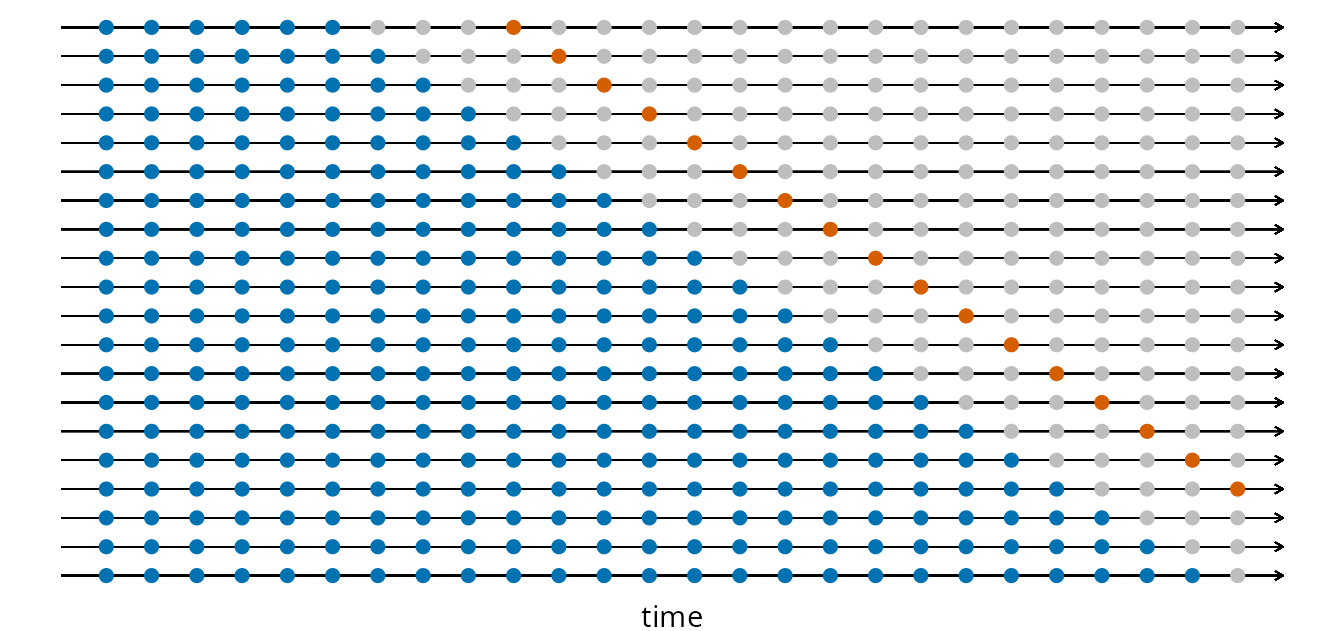
\includegraphics[width=0.48\linewidth]{../images/cross_validation.png}
            \caption{\textit{Illustration of the rolling-origin cross-validation scheme, showing the expanding training set and one-step-ahead test set. \cite{fpp3_CV}}}
      \end{figure}
   
   \subsection{Results}

      \begin{table}[H]
         \centering
         \begin{tabular}{lcccccc}
         \hline
         \multirow{2}{*}{Model} & \multicolumn{3}{c}{RMSE} & \multicolumn{3}{c}{MAE} \\
         \cline{2-7}
         & \multicolumn{3}{c}{Forecasts} & \multicolumn{3}{c}{Forecasts} \\
         & \multicolumn{3}{c}{($h$ day time horizon)} & \multicolumn{3}{c}{($h$ day time horizon)} \\
         & 24 & 168 & 744 & 24 & 168 & 744 \\
         \hline
         Average & {7.731} & \textbf{\textcolor{red}{5.397}} & {7.439} & \textbf{\textcolor{red}{6.042}} & \textbf{\textcolor{red}{4.254}} & {5.385} \\
         Naive & {10.553} & {7.864} & {10.040} & {7.708} & {6.071} & {7.308} \\
         Drift & {10.606} & {8.128} & {11.358} & {7.764} & {6.391} & {8.809} \\
         AR(1) & {8.662} & {5.912} & {8.044} & {6.029} & {4.422} & {5.616} \\
         GP-0-WN & {13.756} & {11.141} & {13.169} & {11.719} & {9.786} & {11.081} \\
         GP-0-SE & {~} & {~} & {~} & {~} & {~} & {~} \\
         GP-MLR-WN & \textbf{\textcolor{red}{7.692}} & {6.134} & \textbf{\textcolor{red}{7.225}} & {6.119} & {4.490} & \textbf{\textcolor{red}{5.136}} \\
         GP-MLR-SE & {~} & {~} & {~} & {~} & {~} & {~} \\
         \hline
         \end{tabular}
         \caption{\textit{RMSE and MAE of forecasting models across horizons.}}
      \end{table}


   \newpage

   \printbibliography

   \nocite{R}

   \section{Appendix}

      \subsection{Code:}

         %\lstinputlisting{R file name.R}

\end{document}
